\documentclass[
10pt,
a4paper,
%parskip=half*, % do not fill last line of paragraph
parskip=half-, % also fill last line of pargaraph until the end
bibliography=totoc,
cleardoublepage=empty,
final,
numbers=noenddot]
%enabledeprecatedfontcommands]
{scrbook}

%\documentclass[10pt, a4paper, parskip=half*, bibliography=totoc, cleardoublepage=empty, final, numbers=noenddot]{scrreprt}	% ongoing pages, no page break after chapter

\renewcommand{\sc}{\scshape}
\renewcommand{\sf}{\sffamily}

%%%%%%%%%%%%%%%%%%%%%%%%%%%%%%%%%%%%%%
%% general
%\usepackage{cmbright} % serifenlose computer modern fonts
\usepackage[T1]{fontenc} % T1 fonts f\"ur gute pdf-Ausgabe
\setkomafont{disposition}{\normalcolor\bfseries} % font for headers same as normal text
\usekomafont{chapter}{\normalcolor\bfseries} % font for chapter headers same as normal text

%\usepackage[ansinew]{inputenc} % wegen deutschen Umlauten
\usepackage[utf8]{inputenc}
% bei mir funktioniert das mit ansinew nicht.  Vermutl. setzt der Editor die Dateien auf utf8, sobald er Umlaute einfügt.  Ich könnte das umstellen, aber eigentlich ist utf8 besser. kai
% hmm, bei mir hat er dann irgendwelche Probleme mit irgendwelchen bibliography Eintr\"agen...

%\usepackage[automark]{scrpage2} % Koma Headers - deprecated....
\usepackage[automark]{scrlayer-scrpage} % Koma Headers - new version
\usepackage[ngerman, english]{babel} % prepare for german AND english, last language loaded is default
\usepackage[autostyle=true, babel, english=american]{csquotes} % babel needs csquotes
%\usepackage{nag} % warn user on outdated packages
\usepackage[linktocpage,pagebackref=true]{hyperref}	% links in pdf, thumbnails
\usepackage{xspace}
\usepackage{diagbox}
\usepackage{soul} % emphasizing text, underlining
\usepackage{breakurl} % for broken urls in Bibliography when hyperref is in use
\usepackage[onehalfspacing]{setspace} % 1.5, change line spaces by \singlespacing \doublespacing
\RequirePackage{fix-cm} 	% error correction for standard fonts
\usepackage[Sonny]{fncychap}	% fancy chapters
\usepackage[titletoc]{appendix}

%%%%%%%%%%%%%%%%%%%%%%%%%%%%%%%%%%%%%%
%% tables
\usepackage{multicol} % multiple columns in tables
\usepackage{multirow} % multiple rows in tables
\usepackage[margin=10pt,labelfont=bf]{caption} % table headers
\usepackage{hhline}	% horizontal lines
\usepackage{longtable} % pagebreak tables
\usepackage{booktabs} % bold table lines, e.g. \toprule
\usepackage{tabularx} % neue Tabular-Umgebung
\usepackage{etoolbox} % adjust font size for tables
\BeforeBeginEnvironment{tabular}{\begin{center}\footnotesize} % adjust font size for tables
\AfterEndEnvironment{tabular}{\end{center}} % adjust font size for tables
%--------------------------------------------------------------------
% table settings
%
\newcommand{\colortableformat}{
	\renewcommand{\arraystretch}{1.3}
	\small
	\sffamily
	\rowcolors{1}{gray!15}{gray!25}% {startrow}{oddrowcolor}{evenrowcolor}
}

%%%%%%%%%%%%%%%%%%%%%%%%%%%%%%%%%%%%%%
%% math, symbols
\usepackage{amsmath} % AMS Math like brackets, integrals...
\usepackage{amssymb} % AMS-Symbols v2.0
\usepackage{fixmath} % big greek letters italic in math mode
\usepackage{array} % matrices
\usepackage{units} % includes nicefrac, nicer fracs for one line, SI-Units
\usepackage{trfsigns} % symbole fÌr transformationen
\usepackage{textcomp} % einfache Sonderzeichen, z.B. \texteuro
\usepackage{gensymb} % correct greek letters in units,\micro instead of \mu
\usepackage[integrals]{wasysym} % for integrals like \oiint
\usepackage[version=3]{mhchem} % easy typesetting of chemical formulae
\usepackage{eurosym} %Eurosymbol

%%%%%%%%%%%%%%%%%%%%%%%%%%%%%%%%%%%%%%
%% graphics
%\usepackage[activate]{pdfcprot} % use margin kerning (character protruding) (Opt. Randausgleich)
\usepackage{microtype} % character protruding, font expansion - instead of pdfcprot
\usepackage{graphicx} % include graphics
\usepackage{wrapfig} % graphics in text
%\usepackage{floatflt} % graphics/tables in text
%\usepackage{rotating} % rotating elements
\usepackage{listings} % for programming source code
\usepackage[svgnames]{xcolor} % colors for listings
\usepackage{psfrag}	% Text in .eps Grafiken ersetzen
\usepackage{subfig}
%\usepackage{subcaption} % can't be used together with subfig
\usepackage{paralist} % in line bullets/points
\usepackage[shortlabels]{enumitem} % different labels for enumerator
\usepackage{bookmark}
\usepackage{tikz}

% clever references, has to be loaded last
\usepackage[capitalise]{cleveref}
\crefname{part}{Part}{Parts}
\Crefname{part}{part}{parts} % only used for ``In this part, ...'' (\nameCref{})
\crefname{chapter}{Ch.}{Chs.}
\Crefname{chapter}{chapter}{chapters} % only used for ``In this chapter, ...'' (\nameCref{})
\crefname{section}{Sec.}{Secs.}
\Crefname{section}{section}{sections} % only used for ``In this section, ...'' (\nameCref{})
\crefname{table}{Tab.}{Tabs.}
\crefname{figure}{Fig.}{Figs.}
\crefname{appendix}{App.}{App.}
\crefname{equation}{Eq.}{Eqs.}

\bookmarksetup{startatroot}
\addtocontents{toc}{\bigskip}% adds a little space in the printed table of contents to visually separate the final chapter from the preceding "part"

% AbstÀnde fÌr Seitenzahlen im Inhaltsverzeichnis erhöhen
\makeatletter
\renewcommand*{\@pnumwidth}{2em} % Breite der Box fÌr Seitenzahlen im Inhaltsverzeichnis erhöhen
\makeatother
%**********************************************

%%%%%%%%%%%%%%%%%%%%%%%%%%%%%%%%%%%%%%
%% bibliography
\usepackage{natbib}
%\usepackage[backend=bibtex,
%			natbib=true,
%			style=authoryear-comp,
%			maxcitenames=2,
%			maxbibnames=99,
%			mincitenames=1,
%			uniquelist=minyear,
%			hyperref=true,
%			arxiv=abs,
%			firstinits=true,
%			mincrossrefs=99,
%			sortcites=false,
%			backref=true]{biblatex}

%%%%%%%%%%%%%%%%%%%%%%%%%%%%%%%%%%%%%%
%% layout
\usepackage[top=4cm,left=3.5cm,right=2.5cm,bottom=4cm]{geometry}

%%%%%%%%%%%%%%%%%%%%%%%%%%%%%%%%%%%%%%
%%%%%%%%%%%%%%%%%%%%%%%%%%%%%%%%%%%%%%
%%%%%%%%%%%%%%%%%%%%%%%%%%%%%%%%%%%%%%

\definecolor{matsimblue}{RGB/cmyk}{50,100,175/0.714,0.429,0.000,0,314}

%% to-do notes
\usepackage[]{todonotes}
%\usepackage[disable]{todonotes}


\def\kmt#1{\textcolor{blue}{[[#1 -- kmt]]}}
\def\kai#1{\textcolor{darkgreen}{[[#1 -- kai]]}}

\def\rewrite#1{\textcolor{teal}{[[#1 -- Umschreiben - ist 1:1 aus Paper]]}}

\newcommand{\kmtTodo}[2][]
{\todo[inline,caption={#2}, size=\scriptsize, color=blue!30, #1]{\renewcommand{\baselinestretch}{0.5}\selectfont#2 KMT\par}}

\newcommand{\kaiTodo}[2][]
{\todo[inline,caption={#2}, size=\scriptsize, color=darkgreen!30, #1]{\renewcommand{\baselinestretch}{0.5}\selectfont#2 KN\par}}

%% mnotes
%\def\mnote#1{\medskip\centerline{\hfill\textcolor{red}{\small #1}}}
\def\mnote#1{\relax}

%%%%%%%%%%%%%%%%%%%%%%%%%%%%%%%%%%%%%%
%%%%%%%%%%%%%%%%%%%%%%%%%%%%%%%%%%%%%%
%%%%%%%%%%%%%%%%%%%%%%%%%%%%%%%%%%%%%%

\graphicspath{{./title/graphics/}{./introduction/graphics/}{./congestion/ptDelayPricing/}{./congestion/congestionPricing/}{./congestion/vtts/}{./noisePricing/noise/}{./noisePricing/ACP/graphics/}{./noisePricing/MCP/}{./severalExternalEffects/simultaneous/}{./congestion/decongestion/}{./severalExternalEffects/cna/}{./avOpt/}}

%%%%%%%%%%%%%%%%%%%%%%%%%%%%%%%%%%%%%%
%%%%%%%%%%%%%%%%%%%%%%%%%%%%%%%%%%%%%%
%%%%%%%%%%%%%%%%%%%%%%%%%%%%%%%%%%%%%%

\makeatother
%--------------------------------------------------------------------
% glossary
\usepackage[toc, acronym]{glossaries}
% !TEX root = ../phd.tex

%%%%%%%%%%%%%%%%%%%%%%%%%%%%%%%%%%%%%%%%%%%%%%%%%%%%%%
%%%%%%%%%%%%%%%%%%%%%%%%%%%%%%%%%%%%%%%%%%%%%%%%%%%%%%
% acronyms
%%%%%%%%%%%%%%%%%%%%%%%%%%%%%%%%%%%%%%%%%%%%%%%%%%%%%%
%%%%%%%%%%%%%%%%%%%%%%%%%%%%%%%%%%%%%%%%%%%%%%%%%%%%%%

%\newacronym[description={Extensible Markup Language, see
	%	\url{www.w3.org/XML}}]{xml}{XML}{Extensible Markup Language}

%Hinweis: die Description  ist nur notwendig, wenn diese von der Langfassung (letztes {}-Paar) abweicht.
%Hinweis:  Pluraldefinitonen sind nur notwendig, wenn diese nicht durch dranhängen eines "s" gebildet werden..

\newacronym{API}{API}{Application Programming Interface}

\newacronym{BEV}{BEV}{Battery Electric Vehicle}

\newacronym{DSL}{DSL}{Domain-specific language}

\newacronym{DRT}{DRT}{Demand responsive transport}

\newacronym{eu}{EU}{European Union}

% \newacronym{FCEV}{FCEV}{\acrlong{FC}  Engine Vehicle}

\newacronym[description={GeoServer is an open source server for sharing geospatial data, see \url{https://geoserver.org}}]
{GeoServer}{GeoServer}{GeoServer geospatial data server}

\newacronym{hbefa}{HBEFA}{Handbook on Emission Factors for Road Transport}

\newacronym{HTML 5}{HTML 5}{Hypertext Markup Language, version 5}

\newacronym[description={Hypertext Transfer Protocol. HTTP and its encrypted version HTTPS are the primary data transfer protocols used by websites}]
{HTTP}{HTTP}{Hypertext Transfer Protocol}

\newacronym{ICEV}{ICEV}{Internal Combustion Engine Vehicle}

\newacronym[description={Java programming language, see \url{www.java.com}}]
{java}{Java}{Java programming language}

\newacronym{KPI}{KPI}{Key Performance Indicator}

\newacronym{lez}{LEZ}{Low Emissions Zone}

\newacronym[description={JavaScript programming language, see \url{www.javascript.info}}]
{JavaScript}{JavaScript}{JavaScript programming language}

\newacronym[description={Multi-Agent Transport Simulation, see \url{www.matsim.org}}, sort=matsim]
{MATSim}{\mbox{MATSim}}{Multi-Agent Transport Simulation}

% \newacronym[description={jsprit, an open-source \acrlong{vrp} - solver, see \url{http://jsprit.github.io/}}]
% {jsprit}{jsprit}{jsprit}

\newacronym{PAVE}{PAVE}{PAVE Project: Potential of Automated Transport Systems}

\newacronym{SPA}{SPA}{Single Page Application}

\newacronym{UI}{UI}{User Interface}

\newacronym{UX}{UX}{User Experience}

\newacronym[description={VSP is Verkehrssystemplanung und Verkehrstelematik, the transport planning and transport telematics chair at Technische Universität Berlin}]
{VSP}{VSP}{Verkehrssystemplanung und Verkehrstelematik, Technische Universität Berlin}

\newacronym[description={Extensible Markup Language, see \url{www.w3.org/XML}}]
{xml}{XML}{Extensible Markup Language}

\newacronym[description={Yet Another Markup Language, see \url{yaml.org/}}]
{YAML}{YAML}{Yet Another Markup Language}

%%%%%%%%%%%%%%%%%%%%%%%%%%%%%%%%%%%%%%%%%%%%%%%%%%%%%%
%%%%%%%%%%%%%%%%%%%%%%%%%%%%%%%%%%%%%%%%%%%%%%%%%%%%%%
% symbols/units
%%%%%%%%%%%%%%%%%%%%%%%%%%%%%%%%%%%%%%%%%%%%%%%%%%%%%%
%%%%%%%%%%%%%%%%%%%%%%%%%%%%%%%%%%%%%%%%%%%%%%%%%%%%%%

\newacronym[description={particulate matter}, %sort={pm},
nonumberlist]{pm}{\ensuremath{\mathit{PM}}}{particular matter}

\newacronym[description={nitrogen oxides}, %sort={nox},
nonumberlist]{nox}{\ensuremath{\mathit{NO_x}}}{nitrogen oxides}

\newacronym[description={sulfur dioxide},
nonumberlist]{so2}{\ensuremath{\mathit{SO_2}}}{sulfur dioxide}

\newacronym[description={non-methane hydrocarbons},
nonumberlist]{nmhc}{\ensuremath{\mathit{NMHC}}}{non-methane hydrocarbons}

\newacronym[description={noise day-evening-night index}, %sort={Lden},
nonumberlist]{Lden}{\ensuremath{\mathit{L_{den}}}}{day-evening-night noise index, see Environmental Noise Directive of the European Union \cite{EU2002END}}

\newacronym[description={carbon dioxide}, %sort={co2},
nonumberlist]{co2}{\ensuremath{\mathit{CO_2}}}{carbon dioxide}

\newacronym[description={kilometer, 1000~\acrshort{m}},
nonumberlist]{km}{\ensuremath{km}}{kilometer}

\newacronym[description={square kilometer, $\acrshort{km}^{2}$},
nonumberlist]{sqkm}{\ensuremath{sqkm}}{square kilometer}

\newacronym[description={meter, the SI base unit of length},
nonumberlist]{m}{\ensuremath{m}}{meter}

\newacronym[description={million, $1 \times 10^6$ },
nonumberlist]{mil}{\ensuremath{M}}{million}

\newacronym[description={thousand, $1 \times 10^3$ },
nonumberlist]{k}{\ensuremath{k}}{thousand}

\newacronym[description={Vehicle Kilometer},
nonumberlist]{vkm}{\ensuremath{vkm}}{Vehicle Kilometer}

%\newacronym[description={Vehicle Hour},
%nonumberlist]{vh}{\ensuremath{vh}}{Vehicle Hour}

\newacronym[description={Ton, 1000~\acrshort{kg}},
nonumberlist]{ton}{\ensuremath{t}}{Ton}

\newacronym[description={kilogram, the SI base unit of mass},
nonumberlist]{kg}{\ensuremath{kg}}{kilogram}
%
\newacronym[description={gram, 1/1000~\acrshort{kg}},
nonumberlist]{g}{\ensuremath{g}}{gram}

\newacronym[description={hour, 60~\acrshort{min}},
nonumberlist]{h}{\ensuremath{h}}{hour}

\newacronym[description={minute, 60~\acrshort{sec}},
nonumberlist]{min}{\ensuremath{min}}{minute}

\newacronym[description={second, the SI base unit for time},
nonumberlist]{sec}{\ensuremath{sec}}{second}

\newacronym[description={utility unit},
nonumberlist]{util}{\ensuremath{util}}{util}

\newacronym[description={Euro},
nonumberlist]{EUR}{\ensuremath{\mathit{EUR}}}{Euro}

\newacronym[description={passenger car unit},
nonumberlist]{pcu}{\ensuremath{\mathit{pcu}}}{passenger car unit}
\makeglossaries
%--------------------------------------------------------------------
%listings (code snippets)
%\usepackage{listings}
%\renewcommand{\lstlistlistingname}{List of Listings}
%\lstset{numbers=left, numberstyle=\footnotesize, numbersep=5pt, basicstyle=\footnotesize\sffamily}
%\lstset{language=Java}
%--------------------------------------------------------------------

%%%%%%%%%%%%%%%%%%%%%%%%%%%%%%%%%%%%%%
%%%%%%%%%%%%%%%%%%%%%%%%%%%%%%%%%%%%%%
%%%%%%%%%%%%%%%%%%%%%%%%%%%%%%%%%%%%%%

% author, title, date of thesis
\newcommand*{\Title}{YY HELLO}

\newcommand*{\Autor}{William A. Charlton}
\newcommand*{\Datum}{Berlin 2022}
\title{\Title}
\author{\Autor}
\date{\Datum}

\newcommand{\tfk}[1]{\textsl{\texttt{#1}}}
\newcommand{\fett}[1]{\textbf{#1}}
\newcommand{\kursiv}[1]{\textit{#1}}
\newcommand{\pbb}{\parbox}
\newcommand{\sst}{\scriptstyle}

% \def\tightlist{}

\providecommand{\tightlist}{%
  \setlength{\itemsep}{0pt}\setlength{\parskip}{0pt}}

\def\umbruch{\clearpage}
\definecolor{darkgreen}{RGB}{0 153 0}

% fÃŒr Standardumgebungen
%\renewcommand{\labelitemi}{*} % AufzÀhlungszeichen definieren

%%%%%%%%%%%%%%%%%%%%%%%%%%%%%%%%%%%%%%%
%%%%%%%%%%%%%%%%%%%%%%%%%%%%%%%%%%%%%%%
%%%%%%%%%%%%%%%%%%%%%%%%%%%%%%%%%%%%%%%
%%%%%%%%%%%%%%%%%%%%%%%%%%%%%%%%%%%%%%%

% Allgemeine Schalter - Änderung von Standardeinstellungen
\frenchspacing								% keine lÀngeren Leerzeichen nach Satzende/AbkÌrzungen mit Punkt
%\setlength{\parindent}{0pt}						% kein Einzug bei neuem Absatz
\setlength{\parindent}{1.5ex}						% kein Einzug bei neuem Absatz
%\setlength{\parskip}{1.5ex plus0.5ex minus 0.5ex}	% Abstand zwischen 2 AbsÀtzen
\setlength{\parskip}{0.25ex plus0.25ex minus 0.25ex}	% Abstand zwischen 2 AbsÀtzen


% verwende das paket setspace statt baselinestretch, Vorteil: AbstÀnde in Fußzeilen und
% listenumgebungen etc. bleiben erhalten
%\renewcommand{\baselinestretch}{1.2}			% Zeilenabstand

% WortabstÀnde optimal einstellen (use instead of \sloppy) - Verhindern von rausragenden Zeilen
\tolerance 1414
\hbadness 1414
\emergencystretch 1.5em %1.5em
\hfuzz 0.3pt
\widowpenalty=10000
\vfuzz \hfuzz
\raggedbottom
\brokenpenalty=10000						% Trennung bei Seitenumbruch

\setlength{\headheight}{1cm} 					% Höhe der Kopfzeile
\addtolength{\footnotesep}{2pt}					% Abstand der Fußnote zur Trennlinie

% Setze Überschriftentiefe
\setcounter{secnumdepth}{3}					% Nummerierung der Kapitel
\setcounter{figure}{4}							% Bilder
\setcounter{tocdepth}{2}						% Gliederungsebene fÃŒr Inhaltsverzeichnis

% Einstellungen fÃŒr Kopf- und Fußzeilen
\pagestyle{scrheadings}       					% nutze scrheader
\clearscrheadings             						% lösche alle vorhandenen header
%\addtokomafont{pagehead}{\normalsize\upshape}  % nichtkursive Kopf-/Fußzeilen
\setheadsepline{.1pt}							% trennlinie oben
\setfootsepline{.1pt}							% trennlinie unten

\automark[section]{chapter}   					% links chapter, rechts section

% variere nach ein-/zweiseitig
\makeatletter
\if@twoside												% bei zweiseitig
	\lehead{\leftmark}             % setze Kapitel linke Seite oben
	\rohead{\rightmark}           % setze Abschnitt rechte Seite oben
	\lefoot{\pagemark}            % Seitennummer unten links
	\rofoot{\pagemark}            % Seitennummer unten rechts
	%\lofoot{\Autor}       		% Name des Verfassers nur linke Seite
\else														% einseitig
	\ihead{\leftmark}            	% setze linke kopfzeile
	\ohead{\rightmark}           	% setze rechte kopfzeile
	\ofoot{\pagemark}             % seitennummer unten rechts
	%\ifoot{\Autor}       		% Name des Verfassers unten links
\fi

% Bei Kapiteln ohne Subsection wird Kapitelname eingeblendet, nutze
% \markright{}, um den \rohead freizulassen

\hypersetup{
			pdftitle={\Title},
			pdfsubject={Dissertation, TU Berlin},
			pdfauthor={Kai Martins-Turner},
			pdfkeywords={agent-based transport simulation; freight transport; emissions; logistics; decarobinazation; elektrification; internalization; agentenbasierte Verkehrssimulation; G�terverkehr; Emissionen, Logistik, Dekarbonisierung; Elektrifizierung},
			pdfdisplaydoctitle = {true},
			pdffitwindow = {true},
			pdfpagelayout = {TwoPageRight},
			pdflang={en},
			colorlinks=true,
			citecolor=matsimblue,
			linkcolor=matsimblue,
			urlcolor=matsimblue,
			bookmarksnumbered=true,
bookmarksdepth=4}

\makeatother

\newcommand{\perf}{\it perf}



% =======================================================
%%%%%%%%%%%%%%%%%%%%%%%%%%%%%%%%%%%%%%
%%%%%%%%%%%%%%%  THESIS START  %%%%%%%%%%%%%%
%%%%%%%%%%%%%%%%%%%%%%%%%%%%%%%%%%%%%%
% =======================================================

\ifdefined\user
\usepackage{geometry}
\geometry{a5paper,left=1mm,right=1mm,top=1mm,bottom=2mm}
%\renewcommand{\familydefault}{\sfdefault}
\renewcommand{\familydefault}{\sffamily}
%%\usepackage[utf8]{inputenc}
\else
\fi

\begin{document}

% =======================================================
%%%%%%%%%%%%%% TO-DOs / Questions %%%%%%%%%%%%%
% =======================================================

\pagenumbering{alph}
\listoftodos
\clearpage

\phantomsection
\addcontentsline{}{chapter}{Allgemeine Notizen / Fragen}
\textbf{{\Large Allgemeine Notizen / Fragen}}

\kmtTodo{A4 oder A5 Format? IK hatte A5...}


\clearpage


\pagenumbering{roman}

% =======================================================
%%%%%%%%%%%%%%%%% Title Page %%%%%%%%%%%%%%%
% =======================================================
\phantomsection
\addcontentsline{toc}{chapter}{Title page}
% !TEX root = ../phd.tex

\thispagestyle{empty}

\begin{flushright}

	\begin{figure}[!h]
  	\begin{minipage}{1.8\linewidth}
	\begin{center}
	
\includegraphics[scale=0.075]{chapters/title/TU-logo-kurz-1c-schwarz.png}
  	\end{center}
  	\end{minipage}
	\end{figure}

	% vertikaler Zwischenraum
	\vspace{20mm}

	% Titel der Arbeit
	\LARGE

	\textbf{\hspace{60mm}\Title} \\[2cm]

	\hrulefill

	\large
	vorgelegt von\\

	% Name des Verfassers
	Dipl.-Ing. \Autor\\
	geboren in Takoma Park, Maryland, USA\\
	\vspace{10mm}

	an der Fakultät V -- Verkehrs- und Maschinensysteme\\
	der Technischen Universität Berlin

	zur Erlangung des akademischen Grades\\
	Doktor der Ingenieurwissenschaften\\
	Dr.-Ing.\\
	\vspace{5mm}

	YY Entwurfsversion \\
	%Diskussionsversion \\
  % genehmigte Dissertation\\
	%D83\\

	\hrulefill

 	Tag der wissenschaftlichen Aussprache: YY \todo{Datum einsetzen} \\

	\vspace{5mm}
	Promotionsausschuss:\\
	Prof. Dr. \todo{Vorsitzende:r}(Vorsitzender)\\
    	Prof. Dr. Kai Nagel (Gutachter)\\
    	Prof. Dr.-Ing. \todo{Gutachter 2} (Gutachterin)\\
     	Prof. Dr.-Ing. \todo{Gutachter 3}(Gutachter)\\
	\vspace{6mm}

	Berlin 2022\\

\end{flushright}
\cleardoublepage

% =======================================================
%%%%%%%%%%%%%%%%% Preface %%%%%%%%%%%%%%%
% =======================================================

% Acknowledgements
\phantomsection
\addcontentsline{toc}{chapter}{Acknowledgements}
% !TEX root = ../phd.tex

% ohne Kopf und Fußzeilen
\thispagestyle{empty}

\chapter*{Acknowledgements}

\textbf{THIS IS STILL JUST PASTED FROM KMT'S -- NEED THE GRANTS FOR COVID, AVOEV/PAVE, others?}

This dissertation was funded in part by the German Research Foundation (DFG) within the projects
\emph{Analyse von Strategien zur vollständigen Dekarbonisierung des urbanen Verkehrs (Project number 398051144)},
\emph{Frachtführer und ihre Interaktionen mit dem Verkehrsfluss (Project number 323900421)} and
\emph{Versender und ihre Interaktionen mit den Transportmärkten (Project number 323864563)},
and in part by the German Federal Ministry of Transport and Digital Infrastructure (BMVI) within the project
\emph{Verbundprojekt: Potenziale Automatisierter Verkehrssysteme (PAVE, FKZ 16AVF2147D)}.

I would like to express my sincere gratitude to Kai Nagel for offering me the opportunity to work in this exciting field of research, their valuable advice and guidance throughout each stage of this dissertation.

I am also very thankful to the following people for their helpful input, insightful comments and fruitful discussions:
Chengqi Lu,
Christian Rakow,
Dominik Ziemke,
Gregor Leich,
Gregor Rybczak,
Ihab Kaddoura,
Janek Laudan,
Jakob Rehmann,
Joschka Bischoff,
Michal Maciejewski,
Ricardo Ewert,
Ruan Gräbe,
Sebastian Müller,
Sydney Paltra,
Theresa Ziemke,
and Tilmann Schlenther.

My thanks also go to Andrea Stillarius, Nadja Dautel and Jakub Wilk for their constant administrative and technical assistance. I would also like to thank the staff members at the Institute of Mathematics who maintained the compute servers.

I thank Santi Rodriguez, Aaron Tatar, and Nicolas Borg for their encouragement, deep patience, and sound advice throughout this research.

Last but not least, I am greatly indebted to my family, in particular to my sisters Suzan and Sonya for emotional support, and my parents Bob and Tez, for buying a very expensive Atari 800 computer "for the family" when I was eleven years old, which set me on a lifelong path of technological discovery.

\newpage

\cleardoublepage

% TOC
\phantomsection
\addcontentsline{toc}{chapter}{Table of Contents}
\renewcommand{\contentsname}{Table of Contents}
\tableofcontents
\cleardoublepage

% Figures
\phantomsection
\addcontentsline{toc}{chapter}{List of Figures}
\listoffigures
\cleardoublepage

% Tables
\phantomsection
\addcontentsline{toc}{chapter}{List of Tables}
\listoftables
\cleardoublepage

% Abstract
\phantomsection
\addcontentsline{toc}{chapter}{Abstract}
\glsresetall
\chapter*{Abstract}

For decades, transport modeling and transport simulation platforms have been coupled with data visualization tools to enable analysts and decisionmakers interpret the voluminous outputs that these simulations produce.

This dissertation documents the development and evaluation of web browser based data visualization techniques that integrate with open-source transport microsimulation tools such as MATSim and ActivitySim. Then it describes a new, complete, and novel open-source web platform that enables transport researchers to produce visualizations and data dashboards to support informed decisionmaking. It is organized into three parts:

\begin{itemize}
  \item Initial experiments using servers for processing and storage, and desktop web browsers for displaying simulation outputs
  \item A rethinking of the approach which eliminates the server-side software and moves almost all functionality into the web browser code, for a set of three project websites
  \item The synthesis of the above techniques into a cohesive and generically useful web-based platform
\end{itemize}

The first part describes several small tools exploring transport microsimulation datasets. Limits on dataset size and processing power inherent in desktop web browser-based solutions are considered. Strengths and weaknesses of the approach are considered in detail.

The second part describes a rethinking of this traditional client/server platform design toward an entirely browser-based system. Three project portals are described and address a wide range of topics from COVID-19 virus propagation to demand-responsive automated vehicle transport systems.

The technologies developed in the earlier parts are synthesized into a cohesive, general web-based platform that is described in the final part. The resulting tool, named ``SimWrapper'', can be used by analysts to assess and compare simulation runs, and also produces data dashboard portals that are suitable for a wide audience.

The dissertation closes with a discussion of the benefits and shortcomings of the web-based data visualization techniques developed as part of this research.

\cleardoublepage

% Zusammenfassung
\phantomsection
\chapter*{Zusammenfassung}

Seit Jahrzehnten werden Verkehrsmodellierungs- und Verkehrssimulationsplattformen mit Programmen zur Datenvisualisierung gekoppelt, um analysiernden Personen und Personen mit Entscheidungsbefugnis in die Lage zu versetzen, die umfangreichen Ergebnisse zu interpretieren, die diese Simulationen produzieren.

In dieser Dissertation wirt die Evaluierung von Webbrowser-basierten Datenvisualisierungstechniken dokumentiert, die mit Open-Source-Verkehrs-Mikrosimulationswerkzeugen wie MATSim und ActivitySim integriert werden können. Anschließend wird eine neue und vollständige Open-Source-Webplattform beschrieben, die es Verkehrsforschenden ermöglicht, Visualisierungen und Daten-Dashboards zur Unterstützung einer fundierten Entscheidungsfindung zu erstellen. Sie ist in drei Teile gegliedert:

\begin{itemize}
	\item Erste Experimente mit Servern für die Verarbeitung und Speicherung von Daten und mit Desktop-Webbrowsern für die Anzeige von Simulationsergebnissen
	\item Eine Überarbeitung des Ansatzes, bei der die serverseitige Software eliminiert und zum größten Teil die gesamte Funktionalität in den Code des Webbrowsers verlagert wird, für eine Reihe von drei Projekt-Websites
	\item Die Synthese der oben genannten Techniken zu einer kohärenten und allgemein nützlichen webbasierten Plattform
\end{itemize}

Der erste Teil beschreibt mehrere kleine Tools zur Untersuchung von Verkehrssimulationsdatensätzen. Dabei werden die Grenzen der Datensatzgröße und der Rechenleistung, die Desktop-Webbrowser-basierten Lösungen innewohnen, berücksichtigt. Die Vorteile und Nachteile des Ansatzes werden im Detail betrachtet.

In dem zweiten Teil Teil beschreibt ein Umdenken von dieser traditionellen Client/Server-Plattform hin zu einem vollständig browserbasierten System. Es werden drei Projektportale beschrieben, die ein breites Spektrum von Themen abdecken, von der Ausbreitung des COVID-19-Virus bis hin zu nachfrageabhängigen automatisierten Verkehrssysteme.

Die in den vorangegangenen Teilen entwickelten Technologien werden zu einer zusammenhängenden, allgemeinen webbasierten Plattform zusammengefasst, die im letzten Teil beschrieben wird. Die Dissertation schließt mit einer Diskussion der Stärken und Schwächen der im Rahmen dieser Forschung entwickelten webbasierten Datenvisualisierungstechniken.

\addcontentsline{toc}{chapter}{Zusammenfassung}
\cleardoublepage

% =======================================================
%%%%%%%%%%%%%%%%% MAIN SECTION %%%%%%%%%%%%%%%
% =======================================================
\pagenumbering{arabic}
\glsresetall

% Introduction
\chapter{Introduction}
\label{Introduction:ch}
% !TeX spellcheck = en_US
% !TEX root = ../phd.tex	

\section{Motivation}
\label{sec:intro-Motivation}
\todo[inline]{Motivation schreiben}

%%%
%%%% 
%%From IK:
%\textcolor{cyan}{The remainder of this \nameCref{Einleitung:ch} is structured as follows. \cref{introduction-sec:pricing} addresses the basic relevant economic concepts of external effects and pricing.
%\cref{sec:research-questions} provides the research questions posed in this thesis. In \cref{sec:research-approach}, the general research approach is presented, including the key features of the agent-based and dynamic pricing approach. An overview of the applied simulation framework is provided in \cref{introduction-sec:matsim}. The outline of this thesis and overview of simulation experiments and applied case studies are given in \cref{sec:outline}.}
%%Ende IK:


\section{Forschungsfragen}
\label{sec:intro-Forschungsfragen}
\todo[inline]{Forschungsfragen}
%%%% 
%%From IK:
%Starting from a more general perspective, the first research question addresses the overall functionality of the proposed pricing methodology:
%Is simulated dynamic pricing a useful approach for the optimization of transport systems?
%%
%In this context, the next research question explores both the effectiveness and effects of the pricing methodology: How do congestion pricing or noise pricing change travel behavior and is there a positive impact on the overall system welfare?
%%
%The following research question directly builds on the previous one and addresses the interrelation of different external effects: How are congestion, noise and air pollution correlated with each other; or, what impact does the pricing of a single external effect have on the others?
%%
%A further research question investigates the design of the simulation-based pricing methodology: What are the implications for the design of a pricing strategy resulting from a simulation framework which allows for real-world case studies and stochastic user behavior?
%%
%Additionally, varying assumptions regarding transport users' travel behavior are tackled: How do simulation results change if transport users' mode choice decisions are incorporated into the transport model?
%%
%Finally, optimal pricing strategies are addressed in the context of innovative modes of transportation: How may simulated dynamic pricing contribute to an improvement of the transport system in regard to the prospect of \glspl{SAV}?

\section{Forschungsansatz}
\label{sec:intro-Forschungsansatz}
\todo[inline]{Forschungsansatz}

\section{Gliederung}
\label{sec:intro-Gliederung}
\todo[inline]{Forschungsansatz}

Diese Arbeit ist wie folgt aufgebaut. \cref{part:Grundlagen} enthält die der weiteren Arbeit zugrunde liegenden Rahmenbedingen und verwendete Software.


%The thesis is structured as follows. \cref{part:congestion} addresses the simulation-based computation of congestion prices in the \gls{pt} mode (\cref{ptDelayPricing:ch}) and car mode (\cref{vtts:ch}, \cref{decongestion:ch}).
%\cref{part:noise} describes the computation of noise damages (\cref{noise:ch}) and noise prices (\cref{internalizationACP:ch}, \cref{internalizationMCP:ch}). In \cref{part:severalExternalEffects}, prices are set accounting for several external effects (congestion and noise in \cref{simultaneous:ch}; congestion, noise and air pollution costs in \cref{cna:ch}). \cref{part:avOpt} addresses optimal pricing strategies for \glspl{SAV}. Finally, \cref{chapter:conclusion} provides an overall conclusion and outlook.
%


\addtocontents{toc}{\bigskip}

\part{Grundlagen und Methodik}
\label{part:Grundlagen}

\chapter{Client/Server Visualization for MATSim}
\label{ch:mathub}
\hypertarget{mathub-abstract}{%
\section{0. Abstract}\label{mathub-abstract}}

There are many tools available for analyzing MATSim transport simulation
results, both open-source and commercial. This research builds a new
open-source visualization platform for MATSim outputs that is entirely
web-based. After initial experiments with many different web
technologies, a client/server platform design emerges which leverages
the advanced user interface capabilities of modern browsers on the
front-end, and relies on back-end server processing for more
CPU-intensive tasks. The initial platform is now operational and
includes several aggregate-level visualizations including
origin/destination flows, transit supply, and emissions levels; as well
as a fully disaggregate traffic animation visualization. These
visualizations are general enough to be useful for various projects.
Further work is needed to make them more compelling and the platform
more useful for practitioners.

\hypertarget{introduction}{%
\section{1. Introduction}\label{introduction}}

MATSim is an open-source framework for implementing large-scale
agent-based transport simulations (Horni, et. al, 2016). MATSim is
widely used for transportation research in academic settings, and is
gaining momentum as a tool ready for practice in real-world planning
contexts.

There are many tools available for analyzing MATSim results, both
open-source and commercial. Typically, analysts can choose either the
free tool OTFVis (Strippgen, 2016) or the commercial software Via
(Rieser, 2016), both of which are desktop software packages requiring
installation as well as a fair amount of technical acumen to operate.
Alternatives to these tools include the more general-purpose desktop
mapping software packages such as QGis and ArcGIS, or statistical
software packages, again all of which require installation and expertise
to use.

As MATSim moves from the confines of academic research to a more
public-facing role, a notable gap is apparent: there are no web-based
interactive tools available for disseminating MATSim data and results.
This creates a challenge for using MATSim in public policy settings: the
only people who can meaningfully examine and explore results are those
who have extensive technical knowledge and access to the specialized
software and large datasets involved.

This research explores one way to fill this gap: building an open
web-based data visualization platform which is specifically designed to
complement MATSim.

\hypertarget{motivation}{%
\section{2. Motivation}\label{motivation}}

The rapid advancement of Internet browsing technologies in the last five
years has enabled the web browser to do things much more
``application''-like than ever before: background processing,
three-dimensional rendering using GPU acceleration, offline support, and
more. The combination of these technologies and their standard
implementations on every popular hardware type and operating system now
makes the web a very compelling platform.

For MATSim research, the question is: could a web browser really be
useful for exploring and delivering results when the datasets are so
large? Answering this question is the primary motivation for this
research. Essentially, has the web become powerful enough for MATSim?

Currently, analysis of MATSim outputs ends up in research reports, PDFs,
video screen-recordings, and presentations. An online dashboard of
results which a user could explore and manipulate would not only be more
interactive, but might also reveal findings that the original analysts
hadn't anticipated.

\hypertarget{requirements}{%
\section{3. Requirements}\label{requirements}}

The research team at Technische Universität Berlin had several ``blank
slate'' discussions before any code was written: meaning, if we could
start at the very beginning and design something completely web-based
and open, what would the bare minimum requirements be for it to be truly
useful? The following requirements emerged from those discussions.

\hypertarget{requirement-1-web-browser-based}{%
\subsection{Requirement 1: Web
browser-based}\label{requirement-1-web-browser-based}}

Given the above-stated motivation and hypothesis that the modern web
platform is ready for large-scale visualization tasks, the most obvious
requirement is that the product of this research must work with any
modern web browser.

Several specific web technologies developed and made widely available in
recent years enable us to perform this research: HTML 5, CSS 3, WebGL,
ECMA Script 6, and Web Workers. Briefly, these technologies are:

\begin{itemize}
\tightlist
\item
  \textbf{HTML 5} improves and standardizes the ``document model'' of
  what constitutes a web page and how it is specified.
\item
  \textbf{CSS 3} is a styling language that enables fine-grained layout
  and styling of individual elements on a page. CSS 3 defines in a
  consistent, standard way the details of elements including color,
  size, layout, and animation of page elements.
\item
  \textbf{WebGL} provides in-browser support for the 3D-accelerated
  graphics capabilities of modern machines.
\item
  \textbf{ECMAScript 6} is an updated (2015) version of the venerable
  Javascript scripting language that has been part of the web platform
  since the early 1990's. Recent versions of Javascript eliminate the
  more problematic aspects of the language and make it easier for
  developers to create bug-free, efficient code.
\item
  \textbf{Web Workers} are a recent (2013) addition to the web platform
  that allow background thread processing for long-running tasks. Before
  Web Workers, there was no way to run truly multi-threaded code inside
  a browser.
\end{itemize}

A complication in web development is that the major web browser vendors
implement these technologies on their own timelines, some much more
rapidly than others. Further complicating things is the reality that end
users do not always upgrade their browsers frequently (or at all). This
creates a landscape where there is a technology adoption curve with a
very long ``tail''. Thus, developers of every web site need to make a
conscious decision about where to draw the line -- choosing necessary
technologies for their site to operate correctly, while knowing that
some users with older browsers will either have a sub-optimal experience
or no access to the site at all.

For this research, we are deliberately exploring the latest
\emph{standard} web technologies, with the expectation that access to
these technologies will become more and more common in the future. Thus,
we are targeting the most recent versions of modern web browsers as of
2019, including Google Chrome, Mozilla Firefox, and Apple Safari. All
three browsers fully support the above-listed technologies, and
importantly, all three auto-update automatically, ensuring that most
users of those browsers stay current as these technologies evolve.

\hypertarget{requirement-2-open-source}{%
\subsection{Requirement 2: Open
source}\label{requirement-2-open-source}}

The entire project, including all front-end (browser) and back-end
(server) code, must be fully open-source.

No proprietary or closed licensing schemes were considered, primarily
because excellent proprietary visualization packages for MATSim already
exist. Creating a competing product would be duplicative and
unnecessary, and would not further the research goal of determining
whether web-based technology is now advanced enough to work with MATSim
outputs. The goal of this research is not to replace existing,
proprietary solutions, but rather to complement them.

The software developed as part of this research is licensed entirely
with the GNU General Public License v3, commonly known as the ``GPL''
(Free Software Foundation, 2007).

This matches the license of MATSim itself. Several other open-source
licenses were considered, including the MIT License and the Apache
Public License, but the benefit of sharing a common license with MATSim
outweighs any perceived benefits of switching to other open licenses.

\hypertarget{requirement-3-use-good-defaults-with-minimal-configuration-and-be-opinionated}{%
\subsection{Requirement 3: Use good defaults, with minimal
configuration, and be
opinionated}\label{requirement-3-use-good-defaults-with-minimal-configuration-and-be-opinionated}}

Since its inception, the web platform has had a relentless focus on
simplicity and smooth user onboarding. Users are accustomed to being
immediately familiar with a site -- often within seconds of their first
interaction. Because of this expectation, it is critical that this
research follow current best practices for user interface (UI) and user
experience (UX). Specifically, that means using familiar UI paradigms
such as navigation bars and breadcrumbs, separating configuration from
usage, limiting settings and options to the bare minimum, and being
``opinionated'', i.e.~encouraging a correct way to accomplish a task.

This approach is dissimilar to some data exploration tools (e.g., QGis
and Via) where extreme configurability is emphasized. Rather than
providing myriad options for details such as scales and color ramps, our
research focuses on choosing good defaults and determining whether that
is sufficient for the software to be useful.

\hypertarget{requirement-4-an-extensible-platform}{%
\subsection{Requirement 4: An extensible
platform}\label{requirement-4-an-extensible-platform}}

Every data visualization use case is different; there is no way to
anticipate how the tool will be used. If the platform is too generic, it
will be not at all useful. Conversely, if only hard-coded visualizations
are created for specific projects, it will be relegated to
``demo-ware'', meaning it is a successful technology demonstration but
not actually useful for real users.

To fulfill this requirement the software platform will need to be
extensible: basic capabilities and templates will be provided, but a
user with some level of coding skill should be able to create new
visualizations that are not anticipated by the researchers.

\hypertarget{initial-experiments}{%
\section{4. Initial experiments}\label{initial-experiments}}

It is no exaggeration to state that the Javascript code library
ecosystem is extremely, enormously large. Thousands of libraries and
packages are available on a common centralized Javascript repository
known as ``NPM'', and there are often multiple packages that do similar
things. As a developer, one must assess and select from these packages
or choose to solve a problem by writing code by hand. Of course these
libraries are of varying levels of popularity and quality.

Based on the requirements laid out above, some initial experiments were
carried out to assess various approaches before committing to a
technology stack.

\hypertarget{visualizing-time-dependent-data-on-a-geographic-map}{%
\subsection{Visualizing time-dependent data on a geographic
map}\label{visualizing-time-dependent-data-on-a-geographic-map}}

Two popular web-based Javascript libraries were tested for displaying
geographic data; Leaflet and Mapbox GL. A simple test case comprised of
MATSim simulation outputs was developed, with the goal of displaying
aggregated roadway link volumes by time of day.

Leaflet (leafletjs.com) is very popular and its application programming
interface (API) is a bit simpler than that of Mapbox GL. Leaflet uses
background map ``tiles'' at specific zoom levels, and layers data on top
of those base maps. With small networks (we tested Cottbus, Germany, a
small city of 100,000 inhabitants) Leaflet performed well, but
medium-sized and large-sized networks with many elements visible at once
suffered from noticeable performance degradation. This was problematic,
as this was the simplest use-case envisioned.

Mapbox GL (mapbox.com) fared much better, apparently better-suited to
displaying large datasets with many visible features simultaneously. In
addition, Mapbox GL's use of 3D vector graphic mapping instead of preset
tiles made for a much more pleasing user experience, with smooth
animations between zoom levels and better background processing during
page loads. For these reasons, Mapbox GL was chosen as the base map for
the remaining geographic visualizations.

\hypertarget{visualizing-non-geographic-data}{%
\subsection{Visualizing non-geographic
data}\label{visualizing-non-geographic-data}}

There are hundreds of data visualization libraries available for the web
which provide ways to produce charts and plots of varying complexity.
Our requirement of using open-source code narrows the field
considerably.

After experimenting with several packages including D3, Raphael, Morris
and others, the package Vega-Lite (Satyanarayan, 2016) exhibited many of
the characteristics desired. Notably, Vega-lite follows a ``grammar of
graphics'' declarative syntax, as popularized by Wilkinson (2005), and
this grammar allows concise description of the meaningful components of
a graphic. An added benefit is that graphs and charts can be downloaded
in image format or in Vega source format, which is helpful for other
researchers wanting to learn how to use the data format themselves.

\hypertarget{dealing-with-large-datasets}{%
\subsection{Dealing with large
datasets}\label{dealing-with-large-datasets}}

MATSim network files are small enough to fit in RAM, but MATSim plan
files and event files can be much larger than RAM, necessitating careful
consideration about how to handle them.

Modern browsers allow access via API to a data storage area that is
unique per hostname, i.e.~http://mysite.com is allowed some storage on
the local machine. Initial experiments revealed that each browser vendor
implements this storage differently, with very strict limits on the
absolute amount storage available, sometimes based on how much free
space remains on the user's machine. It became apparent that this local
browser-based storage would not be sufficient for MATSim outputs.
Running a local file-server process would allow browser access to a
specific folder on the machine, which might be nice for advanced
analysts but violates the research goal of being fully web-based on the
client end. Thus, a client-server paradigm emerges as the only truly
viable alternative, and indeed this is how most websites operate today:
the browser is the front-end to the heavier processing and storage tasks
that happen on someone else's server. Note that ``someone else's
server'' is usually referred to as ``the cloud''.

\hypertarget{platform-architecture}{%
\section{5. Platform architecture}\label{platform-architecture}}

A client/server architecture was chosen for this research based on the
initial experiments described above.

The research team authored back-end server software for file storage,
user authentication, and data pre-processing. Due to space
considerations, this paper does not delve into the details of those
components. Suffice it to mention that the front-end communicates with
them to establish what resources a user has access to, and provides an
application programming interface, or API, with which to query and fetch
available files and resources. The code for those servers is also open
source, and may be the subject of future papers.

The front-end architecture has several interacting components:

\hypertarget{vue-single-page-application}{%
\subsection{``Vue'' Single Page
Application}\label{vue-single-page-application}}

The primary framework used to build the application is known as ``Vue
JS'' (Vue, available at vuejs.org). Vue is a framework for building
interactive user interfaces on the web; essentially it provides the glue
between the items a user clicks and the code that runs when they do so.
Vue provides many services which allow a web page to behave more like a
full-featured application, including state management, routing between
different URLs, and componentization of code in a way that encourages
code reuse and loose coupling. Vue depends on Javascript, which means it
does not work on for users who have disabled scripting in their browser.

Vue is most often used to write so-called ``single page applications''
which are websites that behave like desktop applications. Most large,
popular websites such as Github, Twitter, and Facebook all employ this
paradigm, meaning the site handles page transitions and URL's as if they
are all in one common namespace, and the user thinks less about visiting
URLs and more about navigation through visual components to accomplish
tasks. This matches our use case.

Vue components each encapsulate the three elements required for the
modern web: HTML layout, Javascript code, and CSS formatting. Components
only interact with each other through well-defined pathways of
properties and events, which greatly improves debuggability.

\hypertarget{build-system}{%
\subsection{Build system}\label{build-system}}

The build system of a modern web application is fairly complex and the
Javascript ecosystem changes rapidly. After numerous iterations, the
current build system comprises a series of individual tools that all
work together to produce the final assets that get sent to a user's
browser. Those tools include the Vue command line interface (CLI), the
NPM package manager, webpack, babel, and TypeScript.

Notably, the initial codebase was migrated to the Typescript language
midway through development, as the benefits of a strongly-typed language
were perceived to be worth the development time. TypeScript is a
separate language from JavaScript, and enforces type annotations for
variables and adds additional features such as enumerations. The
TypeScript compiler then converts TypeScript code into ECMAScript 6
JavaScript, which can be run in the browser (as JavaScript is the only
scripting language that browsers support).

\hypertarget{visualization-plug-ins}{%
\subsection{Visualization plug-ins}\label{visualization-plug-ins}}

One of the main requirements of this research is to produce a system
where new visualizations can be produced rapidly and added into the
existing framework to generate new capabilities.

The Vue component architecture enables this. To create a new
visualization, a developer copies an existing ``blank'' visualization
template and gives it a new name, specifies the file inputs and
parameters required, and then uses the above-described libraries to
modify the code per their needs.

This currently requires ample coding skill in Javascript; it is not a
system that is point-and-click like an online data exploration tool.
Experience with other similarly-designed platforms suggests that
software-minded analysts or modelers would be able to extend the
platform, but typical end users will not.

\hypertarget{results-the-current-state-of-the-tool}{%
\section{6. Results: the current state of the
tool}\label{results-the-current-state-of-the-tool}}

A working instance of the platform is now online and available at
https://viz.vsp.tu-berlin.de. Sample datasets are uploaded, and
pre-built visualizations are publicly accessible, as a demonstration of
the platform's current state. There is also a user login system so that
internal researchers can extend and experiment with the system, without
exposing data or work-in-progress to the public.

Basic user, project, and file management capabilities are operational.
This includes grouping files by model run or by other user-defined tags.

Several types of aggregate visualizations are developed:

\begin{itemize}
\tightlist
\item
  Origin/destination flows between aggregate areas, so called ``spider
  diagrams''
\item
  Link flows, by time of day and mode
\item
  Transit supply explorer, which displays all transit routes and allows
  the user to see which routes serve specific stops and links.
\item
  Sankey diagrams, which can be used to depict changes/flows between
  between scenarios across multiple choices, such as shifts in mode
  between two scenarios (see Figure 1d)
\item
  Emissions levels on a geographic hexagonal grid basis
\end{itemize}

In addition, one disaggregate animation is available:

\begin{itemize}
\tightlist
\item
  A vehicle flow simulation, showing individual vehicle agents in
  real-time on the network.
\end{itemize}

See the following screenshots in \emph{Figure 1} for examples of the
current state of the user interface. Note of course that the tool demos
better live than in screenshots, as the whole point of this research is
to develop an interactive tool.

% \begin{figure}
% \centering
% \includegraphics{chapters/02-research/images/all-figures.png.pdf}
% \caption{Sample visualizations, 1a - 1f}
% \end{figure}

\hypertarget{workflow-feedback}{%
\subsection{Workflow feedback}\label{workflow-feedback}}

User interface design (UI) and user experience (UX) have their own
entire fields of research. Initial prototypes of the tool simply did not
meet the needs of test users. Problems included: difficult discerning
which files were which; inability to efficiently use the model run
tagging feature (in which a user could mark sets of files as belonging
to a particular MATSim run); separate user logins causing data to be
inaccesible to team members working on the same projects (resulting in
everyone using a common ``team'' login, against best practices); private
projects ``leaking'' onto the public website; and myriad usability bugs
in the data visualizations themselves.

These usability problems were eventually solved by surveying other
technical websites which organize and present large amounts of data. One
website in particular, Github.com, was found to be well-liked by test
users and has a similar hierarchical view of data: users can belong to
organizations, and both organizations and users can create projects
(``repositories'' on Github) which may large numbers of files.

By adopting a file, project, and user paradigm similar to that employed
by Github, users were immediately more familiar and had less to learn.
The current site adheres to this so closely that test users often refer
to the platform as ``MatHub''.

\hypertarget{performance}{%
\subsection{Performance}\label{performance}}

Even with modern hardware and the latest browsers, it is quite
challenging to produce performant, visually pleasing results with
disaggregate MATSim data. The vehicle flow simulation depends heavily on
the back-end server to produce and deliver simulation ``frames'' to the
browser in real-time, so that the browser simply has to render the data.

Various levels of aggregation make MATsim data much easier to visualize,
as is reflected in the number of different visualizations this research
was able to produce with aggregate data in a short time frame.

\textbf{Preprocessing.} The traffic animation and the emissions ``hex
grid'' visualizations both rely on back-end server processes to
preprocess the raw MATSim event outputs. This takes anywhere from a few
seconds to many minutes, depending on the size of the simulation that
was run. The preprocessing only needs to occur once, and thereafter the
results are cached and stored on the server. The UI presents a helpful
``still processing'' message during this stage. Unfortunately, changing
some settings such as the size of the hex-grids for the emission tool
means the calculations must be redone. Further work is being done to
make these processes run as quickly as possible.

\textbf{Map layer limitations.} The Mapbox GL mapping library allows
lines, points, and polygons to be displayed on top of a base map. There
seems to be a number of map elements beyond which performance becomes
very slow; various techniques can be used such as aggregating elements
at further-out zoom levels to get around this. Another option is to only
use Mapbox GL for the base map, and to use the WebGL graphics libraries
to draw large numbers of elements directly on top of the map. This is
the technique used for the traffic animation, which can easily support
tens of thousands of elements (all in motion!) simultaneously. For
additional visualizations which have large numbers of grahical elements,
more research will need to be done on layering WebGL elements on top of
the base map.

\hypertarget{mobile-device-support}{%
\subsection{Mobile device support}\label{mobile-device-support}}

Initially, the research targeted desktop browsers only. The reasoning
was that analysts currently use desktop software, and it would be
sufficient to complement those desktop tools with a new web-based
option.

However, as the tool started becoming usable by internal users, it
quickly became apparent that everyone wanted some version of the
visualizations to work on mobile devices, too. It was suggested that
even a read-only visualization ``viewer'' for mobile would be better
than not having the tool work at all on mobile.

To address this, the layout of the main user interface needed to be
redesigned, but the overall stack of web-based libraries and components
chosen was already well-suited to mobile use. This effort is currently
underway.

\hypertarget{conclusions-and-outlook}{%
\section{7. Conclusions and outlook}\label{conclusions-and-outlook}}

Experimenting with the various technologies and getting all of the
disparate pieces working together was an enormous task, one which took
much longer than anticipated. However, those decisions are now behind us
and the platform has become quite stable.

A new visualization can now be generated by the researchers in a matter
of days or weeks. The researchers are admittedly very familiar with the
inner workings of the system, but even so it has been encouraging to see
new visualizations go from ideation to rough draft in such a short time.

None of the above-listed visualizations are particularly groundbreaking
or visually stunning. And, all of them could be easily created in other
tools (although usually without the interactivity that the web enables).
This is a bit disappointing but the open nature of the platform,
requiring no software installation by end users, still has an advantage:
it opens up the display of MATSim results to the public and to
decisionmakers, even if they do not have access to desktop mapping or
travel forecasting software.

Another use case that has emerged from these visualization experiments
is a more regimented data management tool for MATSim. Currently there is
no straightforward way to share MATSim datasets online. The combination
of the new file storage and management capabilities along with the
Github-like user interface provides a natural place for users to store
and disseminate results.

Importantly, the world has not stood still while this platform was under
development. Just in the past year, major data visualization efforts
from well-funded companies such as Uber and others have been released.
There are legitimate questions about how much of this work could be
superceded by large, well-funded, professional coding teams.

Despite these concerns, the MATSim visualization framework is
operational and is now just beginning to be useful for researchers at
the department of its creation. This bodes well for further development
in the near future.

All code is available on the MATSim Github site, at
https://github.com/matsim-org/viz.

\hypertarget{references}{%
\section{References}\label{references}}

GNU General Public License (June 29, 2007). Version 3. Free Software
Foundation. URL: https://www.gnu.org/licenses/gpl.html

Horni, A., Nagel, K. and Axhausen, K.W. (eds.) 2016 The Multi-Agent
Transport Simulation MATSim. London: Ubiquity Press. DOI:
http://dx.doi.org/10.5334/baw. License: CC-BY 4.0

Rieser, Marcel (2016): Senozon Via. In Andreas Horni, Kai Nagel, Kay W.
Axhausen (Eds.): The Multi-Agent Transport Simulation MATSim: Ubiquity
Press, pp.~219--224.

Satyanarayan, A., Moritz, D., Wongsuphasawat, K., and Heer, J. (2016):
Vega-Lite: A Grammar of Interactive Graphics. IEEE Transactions on
Visualization and Computer Graphics, Volume 23, Issue 1. DOI:
https://doi.org/10.1109/TVCG.2016.2599030

Strippgen, David (2016): OTFVis: MATSim's Open-Source Visualizer. In
Andreas Horni, Kai Nagel, Kay W. Axhausen (Eds.): The Multi-Agent
Transport Simulation MATSim: Ubiquity Press, pp.~225--234.

Wilkinson, Leland (2005): The Grammar of Graphics, Second Edition.
Springer Press, Chicago, USA. DOI: https://doi.org/10.1007/0-387-28695-0


\chapter{COVID-Sim}
\label{ch:covid-sim}
\hypertarget{introduction-covid-19-and-episim}{%
\section{Introduction: COVID-19 and
EpiSim}\label{introduction-covid-19-and-episim}}

In February 2020, the team at VSP began work on an extension to MATSim which soon became known as ``EpiSim.''

YY reference which paper/papers?

The EpiSim model was a novel hybrid of the agent-based microsimulation model MATSim and epidemiological infection progression models. New versions of the combined model were being released, tested, and run multiple times per week in the frenetic early days of the COVID-19 pandemic in Europe. This produced massive amounts of data from literally hundreds of model simulations -- often daily.

It quickly became apparent that the team needed a way to compare all of these runs in a visual manner, and also to be able to convey salient results to decisionmakers and the public. A web-based solution was an obvious choice for both use cases, but the many problems we encountered in modifying or enhancing MatHub made us unsure that a heavyweight client/server solution would be able to keep up with the team's needs.

We decided to take an unusual approach for such a large undertaking, which leveraged the investments already made in web-based visualization technologies but jettisoned all of the back-end servers: we rapidly built what is called a ``Single Page Application'' (SPA) that was a completely self-contained website, with no back-end server processing at all. All of the website code and all of the data files would be served ``statically'' from a simple web server.

Eventually the size of the site expanded and the data storage for model results was moved to a dedicated file server, but otherwise the overall architecture remained constant and the site continues in operation today.

This approach proved successful in meeting our team's needs, and is described fully in this chapter.

The COVID-Sim website is available at \url{https://covid-sim.info}

\hypertarget{how-websites-are-built-clients-and-servers}{%
\subsection{How websites are built: clients and servers}\label{how-websites-are-built-clients-and-servers}}

As described earlier in YY, web sites always consist of the content which is loaded into a browser, known as the ``client'', and the back-end servers which the client connects to. In the simplest case, a user points to a URL, and the browser loads the HTML index file at that location along with any other static files referenced in the HTML. This is known as a ``static'' website, as the web server doesn't need to do any dynamic processing to serve the request; it simply delivers the requested files over the network.

Of course, much more complex arrangements are also possible. The web server can run code or scripts which generate part of the page dynamically, can call APIs which pull data from other servers or databases, and so on. These are known as ``dynamic'' sites, and for example our MatHub project used this arrangement.

\hypertarget{single-page-applications}{%
\subsection{Single Page Applications}\label{single-page-applications}}

As early as 2003 {[}YY reference SPA page on wikipedia -- better ref?{]}, the concept of a single-page application which runs Javascript code in the browser was already in existence. These types of sites run Javascript locally in the browser to transform the page contents that arrive from the web server. This is often done to make a page feel more interactive or more like a native desktop app. Some of the most popular websites in existence, such as Twitter and Facebook, employ this architecture.

Contrast this with the more traditional client/server architecture that frameworks such as PHP or Ruby on Rails employ: a network request from a browser client results in code running on the server which then builds and returns an HTML page to the client.

Crucially, the SPA approach allows for user interactions to modify the content of a page without requiring a round-trip data request to a support server. Once the page is loaded, the SPA is ready. Further API calls are allowed, of course, which means data can be queried from external sources as needed. But the essential Javascript code which drives the website functionality is delivered to the browser and runs there.

\hypertarget{the-episim-single-page-application}{%
\section{The EpiSim Single Page Application}\label{the-episim-single-page-application}}

This approach seems ideal for our needs, as we didn't want to be modifying server code every time a new version of the EpiSim model added new parameters.

Thus we created our first simple Vue-based YY single page application which loaded a basic HTML template, a zipfile with all summary model run outputs, and the view logic to link a few slider bars with pandemic intervention approaches with some resulting line charts of pandemic progression over time.

YY show pic of v1

The initial interventions being considered were: ``Close Public Transit'', ``Close Workplaces'', ``End Social Activities'', and ``End All Other Activities''. Each of these interventions could be user-selected at a given timepoint, measured from ``Never'' to 10, 20, or 30 days after the start of the pandemic. Notably, these were the early days before many other measures such as mask mandates, school closures, or eliminating air travel were available -- and vaccination programs were still far off in the future.

The site was operational internally in a matter of days, and made public on March 30, 2020.

The first versions of the site were produced rapidly and were quite crude, for example with no overall site navigation and almost nothing in terms of exposition. As the project (and pandemic) continued, more model versions were developed and each previous version was archived (but accessible) for reference and comparison.

\hypertarget{cataloging-model-input-parameters-and-the-resulting-model-outputs}{%
\section{Cataloging model input parameters and the resulting model outputs}\label{cataloging-model-input-parameters-and-the-resulting-model-outputs}}

As EpiSim gained complexity, so did the model output portal. The number of simulations ballooned to hundreds or thousands of runs per week, and new versions of the model itself were developed to improve results and to answer decisionmaker questions about the latest turns of the pandemic -- whether that be mask mandates, school closures, vaccination strategies, boosters, etc.

To keep up with this churn, the data visualization strategy was also constantly modified. In particular, a new way of mapping the multitude of inputs to the run identification numbers (``Run IDs'') was developed, as the initially small handful of four slider bars was quickly replaced by groups of numerous buttons grouped into logical sets, every combination of which would reference one specific model run.

The combinatorial nature of these options made it imperative that we adopt an automated process for identifying model outputs, as well as a way to navigate between different versions of the model itself.

\hypertarget{describing-simulations-using-yaml}{%
\section{Describing simulations using YAML}\label{describing-simulations-using-yaml}}

The solution is comprised of two pieces of data for each batch of model runs:

First, a simple table that links the run identification numbers with the specific input parameter values for every parameter in the model. So for a batch of runs testing four mask strategies and two school closure strategies, 4x2 is eight combinations of parameters, thus the table includes eight rows. Each row assigns a Run ID and the value of the two hypothetical parameter values. In reality there are always far more than eight combinations; often 768 or 1,024 different permutations of a dozen parameters were tested, all batched together in a nightly run on the University high-performance compute cluster. This lookup table is stored as a simple text file in CSV format.

Second, for the display of available options to users of the EpiSim dashboard, a human-friendly mapping between option groups, variable names, and values is needed.

Most variables in EpiSim are either general in nature, affecting the entire simulation; or time-based, occurring on specific dates or ``X days after'' the start of the simulation. This leads to a natural grouping of parameters which makes the many user interface options more digestible for non-experts in EpiSim.

The EpiSim parameters themselves are usually numeric or categorical; each variable can have multiple values that also have a human-interpretable meaning. For example the percentage of people wearing masks on transit; or the types of masks being worn (N95, surgical, none).

Capturing all of this information in a definable, repeatable format for use in the user interface required something more structured than the simple lookup table above.

For this, we use a common configuration file format known as YAML (``Yet another markup language''). The YAML standard is defined at YY.

YAML excels at describing sets of key:value relationships. It is human-readable and computer-parseable; these traits lead to YAML being a common format for specifying configuration information.

YY Ask Christian - how does this work

For a batch of EpiSim runs, the operator of EpiSim produces the lookup table with the specific model parameters and a YAML file containing the metadata that describes in human terms how the variables will be presented to the user in the dashboard.

An example YAML file is below: this is abbreviated for clarity. More complex model runs have more sections and more variables defined.

YY

\hypertarget{retrieving-model-results}{%
\section{Retrieving model results}\label{retrieving-model-results}}

The final piece of the puzzle is the storage and retrieval of the actual model results.

A batch of simulation runs produces summary outputs for every combination of model parameters. Those outputs are identified by the Run ID defined above, and they are compressed into a single .ZIP format file archive. The contents of the .ZIP file vary based on what version of the model was run: early versions only included YY, while later versions added additional outputs such as YY.

Thus a full batch output, ready for display in the COVID-Sim website,
includes:

\begin{itemize}
\item
  info.txt: the table of simulation Run IDs along with the specific
  values for every model parameter used; one row per simulation.
\item
  metadata.yaml: the collection of descriptive names for each variable
  and their groupings
\item
  summary zip files: a folder containing one .ZIP file for each
  simulation.
\end{itemize}

These files are stored on the departmental file server in hierarchical folders, organized by run date, city, and sometimes other categories.

The COVID-Sim website maps the requested URL directly to the file structure on disk: so for example, http://covid-sim.info/2021/11/05/example-run displays results stored in the 2021/11/05/example-run folder on the file server.

\hypertarget{architecture}{%
\section{Architecture}\label{architecture}}

With all these pieces in place, the unique overall architecture of the EpiSim data visualization portal emerges:

\begin{itemize}
\item
  An ``SPA'' single page application, based on Vuejs and hosted on a
  static website hosting provider
\item
  Hierarchical file storage on a university departmental file server,
  with data for all published runs available via HTTP. Each run is
  stored in its own folder, and contains:

  \begin{itemize}
  \item
    Automatically-generated configuration files, produced when the
    EpiSim simulation runs are set up, which describing the specific
    combinations of input parameters that are to be run.
  \item
    A lookup table which maps each combination of input parameters to a
    specific output dataset
  \item
    Zipped output files containing the summary data for each simulation
    run identifiable in the above lookup table.
  \end{itemize}
\end{itemize}

\ldots{} YY

\hypertarget{animations-of-infection-progression-in-berlin}{%
\section{Animations of infection progression in Berlin}\label{animations-of-infection-progression-in-berlin}}

A second goal of the site was to be an external-facing portal for educating decisionmakers, the media, and the public. Internal analysts much appreciated the ability to compare results of model runs by flipping switches and sliders and seeing how the model output graphs reacted. But as the team took results to non-experts, we identified the need to take a step back and create a visual representation of how the model actually worked.

The agent-based model is based on the daily activities and movements of every population member, interacting with each other, spreading the infection when contagious, and then having the disease progress.

This is well-suited to an animation of the agents moving through time and space. Such an animation was included between versions 2 and 4 of the EpiSim model itself. It depicts the ``do nothing'' scenario for Berlin: how the COVID-19 pandemic would proceed through Berlin and the surrounding areas if no measures at all were taken.

YY some screenshots of the pandemic animation

The infection status of each agent is represented by color: susceptible, infected, contagious, sick, seriously sick (hospitalized), critical (intensive care), and recovered. Their motions can be seen over the course of a day and over the 90-day course of the pandemic simulation. Any specific day in the simulation can be chosen from a panel to see the infection status of the population on that day.

The exponential nature of the pandemic is very clearly illustrated in this manner.

YY Based on feedback, this animation was helpful in the spring of 2020 to help describe how the model worked.

A second animation was added later that removed the daily back-and-forth motion of agents on individual trips, and simply showed the status of agents at their home locations, over the course of the 90-day simulation.

\hypertarget{informing-decisionmaking-with-comparison-dashboards}{%
\section{Informing decisionmaking with comparison dashboards}\label{informing-decisionmaking-with-comparison-dashboards}}

YY How did government get involved ?

Over the twisting course of the COVID-19 pandemic, the EpiSim model acquired new capabilities. Each passing month introduced new questions:

YY timeline:

\begin{itemize}
\item
  masks
\item
  schools
\item
  lockdowns
\item
  events
\item
  dining
\item
  sports
\item
  vaccination
\item
  external travel
\item
  variants
\item
  boosters
\end{itemize}

And the model dashboard grew longer and longer to display new graphs of the salient questions of the day. This iterative process was entirely needs-based: as the team was asked (or anticipated) new questions

\hypertarget{user-feedback}{%
\section{User feedback}\label{user-feedback}}

\hypertarget{iteration-and-further-work}{%
\section{Iteration and further work}\label{iteration-and-further-work}}

\hypertarget{discussion}{%
\section{Discussion}\label{discussion}}


\chapter{AVÖV and PAVE}
\label{ch:pave}
We describe a unique, web-based data visualization portal developed for use by researchers and public transit agencies investigating future shared-taxi fleet scenarios. Augmenting or even replacing fixed-route transit lines with automated, connected, shared taxi fleets may be a desirable alternative in less-densely developed areas. The MATSim agent-based transport microsimulation model is used to study scenarios including the status quo, dynamically-dispatched fleets with drivers, and fully autonomous fleets. This paper focuses on a data visualization portal which includes many interactive views such as agent (taxi) movements color-coded by number of passengers and trip request origins and destinations, changes in roadway and passenger volumes compared to a base case, and more. The agent-based simulation covers a 24 hour simulation period; analysts can hone in on specific times of day to examine, e.g. school pickup/drop-offs or commute trips connecting to rail stations. The tool is in operation for several small cities and rural regions in Germany and was successfully used as an outreach tool in public meetings. In addition, developers of the MATSim DRT extension found the visualizations particularly useful for debugging both the algorithms and the scenario definitions. The code is entirely open source and, while this specific study has a rather esoteric use case, the visualization platform has an extensible design that could be modified for other purposes.

%% ----- INTRODUCTION -----
\section{Introduction}
\label{introduction}

Augmenting or replacing fixed-route transit lines with automated, connected, shared taxi fleets may be a desirable alternative for transit agencies in less-densely developed areas. The economics of fixed-route transit are difficult to square with sparse development patterns, especially with the advent of private ride-hailing services which add the "shared taxi" concept to people's travel options \cite{Hough2018}. The same technologies used by private ride-hailing, however, can also be modified and applied to future transit services.

In this study, known in German as AVÖV\footnote{Automasierter vernetzter öffentlicher Verkehr: Automated, networked public transit}, a new dynamic-response shared taxi service, or "DRT", is examined as an alternative approach to serving the population of rural areas and less-dense portions of urban regions. Dynamic-response transit is analyzed using the MATSim agent-based transport microsimulation model. MATSim is an extensible, activity- and multi-agent based transport simulation, which enables the simulation of large scale scenarios. \cite{MATSimBook}. Crucially, MATSim simulates passenger transport in both private and public modes \cite{ZiemkeEtAl2019OpenBerlinScenario}.

The existing methodology behind using MATSim to simulate DRT is well-described by Bischoff et al \cite{Bischoff2020,BischoffMaciejewskiNagel2017SharedTaxiIITSC} and is not the focus of this paper. Rather, in the course of the effort to develop, analyze and compare various DRT scenarios, a need arose to create some truly unique data visualizations that could assist in improving and displaying the DRT scenarios themselves. A web-based portal is the result of this research. The portal includes many interactive views, such as taxi movements color-coded by number of passengers and trip request origins and destinations, changes in roadway and passenger volumes compared to a base case, and more. The agent-based simulation covers a 24 hour simulation period; analysts can hone in on specific times of day to examine, e.g. school pickup/drop-offs or commute trips connecting to rail stations.

The tool is in operation for several small cities and rural regions in Germany, and was successfully used as an outreach tool in public meetings online. Project partners at transit agencies are interested in understanding the implications of the DRT simulations, and without a visual component, that would be extremely difficult to provide.

Furthermore, developers of the MATSim DRT extension found the visualizations particularly useful for debugging both the algorithms and the scenario definitions. The latest implementions of MATSim include extensive DRT capabilities whose methods are continually being optimized and improved.

All code for MATSim and the visualization portal is open source and, while this specific study has a quite esoteric use case, the portal has an extensible design that could be modified for other purposes.

%% ----- EXISTING TOOLS AND RESEARCH -----
\section{Motivation: Existing Tools and Research}
\label{motivation}

Agent-based microsimulation is quite complex, producing reams of data and overwhelming details that are not appropriate for stakeholder meetings. PDF reports and PowerPoint slides are the norm in these situations, but building something truly interactive instead could be much more engaging and useful for decision-making.

Many existing tools can analyze agent-based transport simulation outputs. \textbf{OTFVis} \cite{Srippgen2015OTFVisInBook} is a venerable open-source tool designed to integrate tightly with MATSim, however it is not under active development and has neither online features nor DRT-specific capabilities.

The commercial product \textbf{Senozon Via} \cite{Rieser2015SenozonViaInBook} is very feature rich, actively maintained, and is currently used by our research team for myriad internal analysis tasks. It has no online web-based component, although it is very easy to create high-quality screen recordings of simulation results. The lack of interactive options for outreach meetings, as well as Via's focus on advanced analyst tasks, make it a poor fit for outreach despite its many other advantages.

General geographic information system tools, such as \textbf{ArcGis} and its open source corollary \textbf{QGis}, are again very analyst-focused. Unlike QGis, ArcGis can create high quality online dashboards and interactive maps, and the study team has used them in other settings. ArcGis does not have any MATSim-specific capabilities; the rich agent-based details would be entirely lost in the aggregations required to get DRT outputs onto an ArcGis map. ArcGis is also commercial software and was not considered due to the required financial outlay.

Research by \citet{CharltonLaudan2020WebBasedVisualization} shows that a web-based tool specific to MATSim is now possible, given the latest advances in graphic technology embedded in modern web browsers. That tool includes a "front-end" website which runs in the user's browser. Through this site the user organizes model outputs, and defines aggregate visualizations for a few typical use cases. The tool also requires a large, complex "back-end" server component which handles file storage, user authentication, output post-processing, and realtime visualization support. That work is an obvious starting point for this research, but for reasons that will be described below, much of it was ultimately discarded.

In summary, the existing tools are all either incapable of visualizing the disaggregate outputs of the DRT module of MATSim in an efficient manner, have no web-based online component, or are inappropriate for anyone except highly trained analysts. Thus the new platform described below is seen as a viable solution.

%% ----- THE PLATFORM -----
\section{The Visualization Platform}
\label{platform}

Despite two years of development of the above-mentioned client/server solution for other studies, problems in the old system are persistent. The two largest: (1) The massive size of MATSim outputs always preclude loading them into a user's web browser; a single DRT run can be 800Mb or more. This forces post-processing and/or aggregation to happen, which can eliminate many of the benefits of a fully disaggregate analysis. (2) The back-end server design requires extensive effort whenever new visualization capabilities are desired. A strict database design and overwrought user/group management capabilities result in a rock-solid system that is extremely onerous to modify.

It turns out that complex file and user management is unnecessary.\footnote{This invokes the programming mantra "YAGNI" -- You Aren't Gonna Need It: build the simplest possible solution that works, instead of over-engineering things.} From trial and error and iteration emerges a simplified system that eliminates all of the back-end server complexity by eliminating all of the back-end servers:

\begin{itemize}
  \item File storage is delegated to existing servers, instead of creating a special visualization file server. On site, we have an existing "Subversion" server \cite{Collins-SussmanEtc2008SubversionBook} which is adept at large-file storage and version history. All access to the server is via a simple interface that can be easily extended to cloud storage, such as Amazon S3
  \item As the site is intended to be publicly accessible, we discard all user authentication capabilities. If you have a web browser, you can view the results of any runs which are stored \emph{in the public area} of the Subversion server. Naturally some parts of file storage remain off-limits to the greater Internet
  \item Analysts define visualizations by creating small configuration text files in the same folder as model outputs. These files include all of the details of a visualization --- usually just a few lines --- pointing to the input files and configuration settings. This eliminates all the hassle of writing code for user interface input dialog boxes.
  \item Post-processing of outputs must be performed by the analyst as part of their modeling workflow, before uploading to Subversion, since browsers cannot ingest MATSim outputs in their entirety. This tool is not an "end-to-end" GUI which lets analysts define, run, and view outputs of their simulations: it is an output viewer.
\end{itemize}

The code is designed as a "Single Page Application" or "SPA" which is a modern way of building Javascript-based websites that behave similarly to desktop applications. Most large consumer websites such as Twitter and Facebook behave in a similar manner, thus this paradigm is easy for end users to understand.

Again after much trial and error for which there is no space in this brief paper, the platform is the combination of many different advanced web technologies:

\begin{itemize}
  \item The overall application framework is based on \textbf{VueJS}, a popular Javascript toolkit for building interactive websites. VueJS is the glue between user interface clicks and the application code that runs underneath.
  \item The agent-based visualizations use custom code ("shaders") written using the \textbf{Deck.gl} visualization library
  \item Older visualizations borrowed from Charlton et al's previous research use the \textbf{Mapbox GL} mapping library
  \item Extensive optimization of memory usage for handling these large datasets with the brilliant \textbf{crossfilter} Javascript library, which manages lightning-fast filtering of millions-of-rows datasets in multiple dimensions
\end{itemize}

The entire codebase is open source and is designed with a "plug-in" architecture so that new visualizations can be developed quickly while relying on common infrastructure for things like file access. To create a new visualization, the developer copies an existing template, modifies the Javascript code to take advantage of the Deck.gl or MapBox libraries as needed, and registers it with the main application. End users can then create visualizations by adding corresponding configuration files to a scenario's file server folder.

%% ----- DRT VISUALIZATIONS -----
\section{Dynamic-Response Taxi Visualizations}
\label{drtviz}

Several unique visualizations depict details specific to the dynamic-response transit scenarios in this study. Standard MATSim outputs such as mode shares by time of day, simulation statistics, trip length summaries, and so on are also available in each scenario subfolder.

The descriptions below fit in the paper's length, but for best understanding of an interactive website, it is better to view the site in situ. The project site remains online and is better demonstrated than described.\footnote{Site is viewable at \href{https://avoev-vsp.github.io}{avoev-vsp.github.io}}

\subsection{DRT Animation}

A 24-hour agent-based interactive animation of DRT vehicles traversing the roadway network includes the following features: (1) DRT vehicles traversing the roadway links in real-time, sped up, or in reverse time, for analysis; (2) Vehicles color-coded by occupancy, so users can see the relative amount of ride-sharing occurring at different times of day; (3) Passenger origin/destinations depicted as "flyovers" instead of on the street network, so actual supply and demand can be viewed separately from the roads on which that demand occurs;

Each of these components can be turned on or off to assist in reducing clutter in the animation. The 3D map can be zoomed or panned and its pitch angle adjusted to assist in viewing.

\begin{figure}[ht]
\centering
\begin{minipage}[c]{0.4\textwidth}
   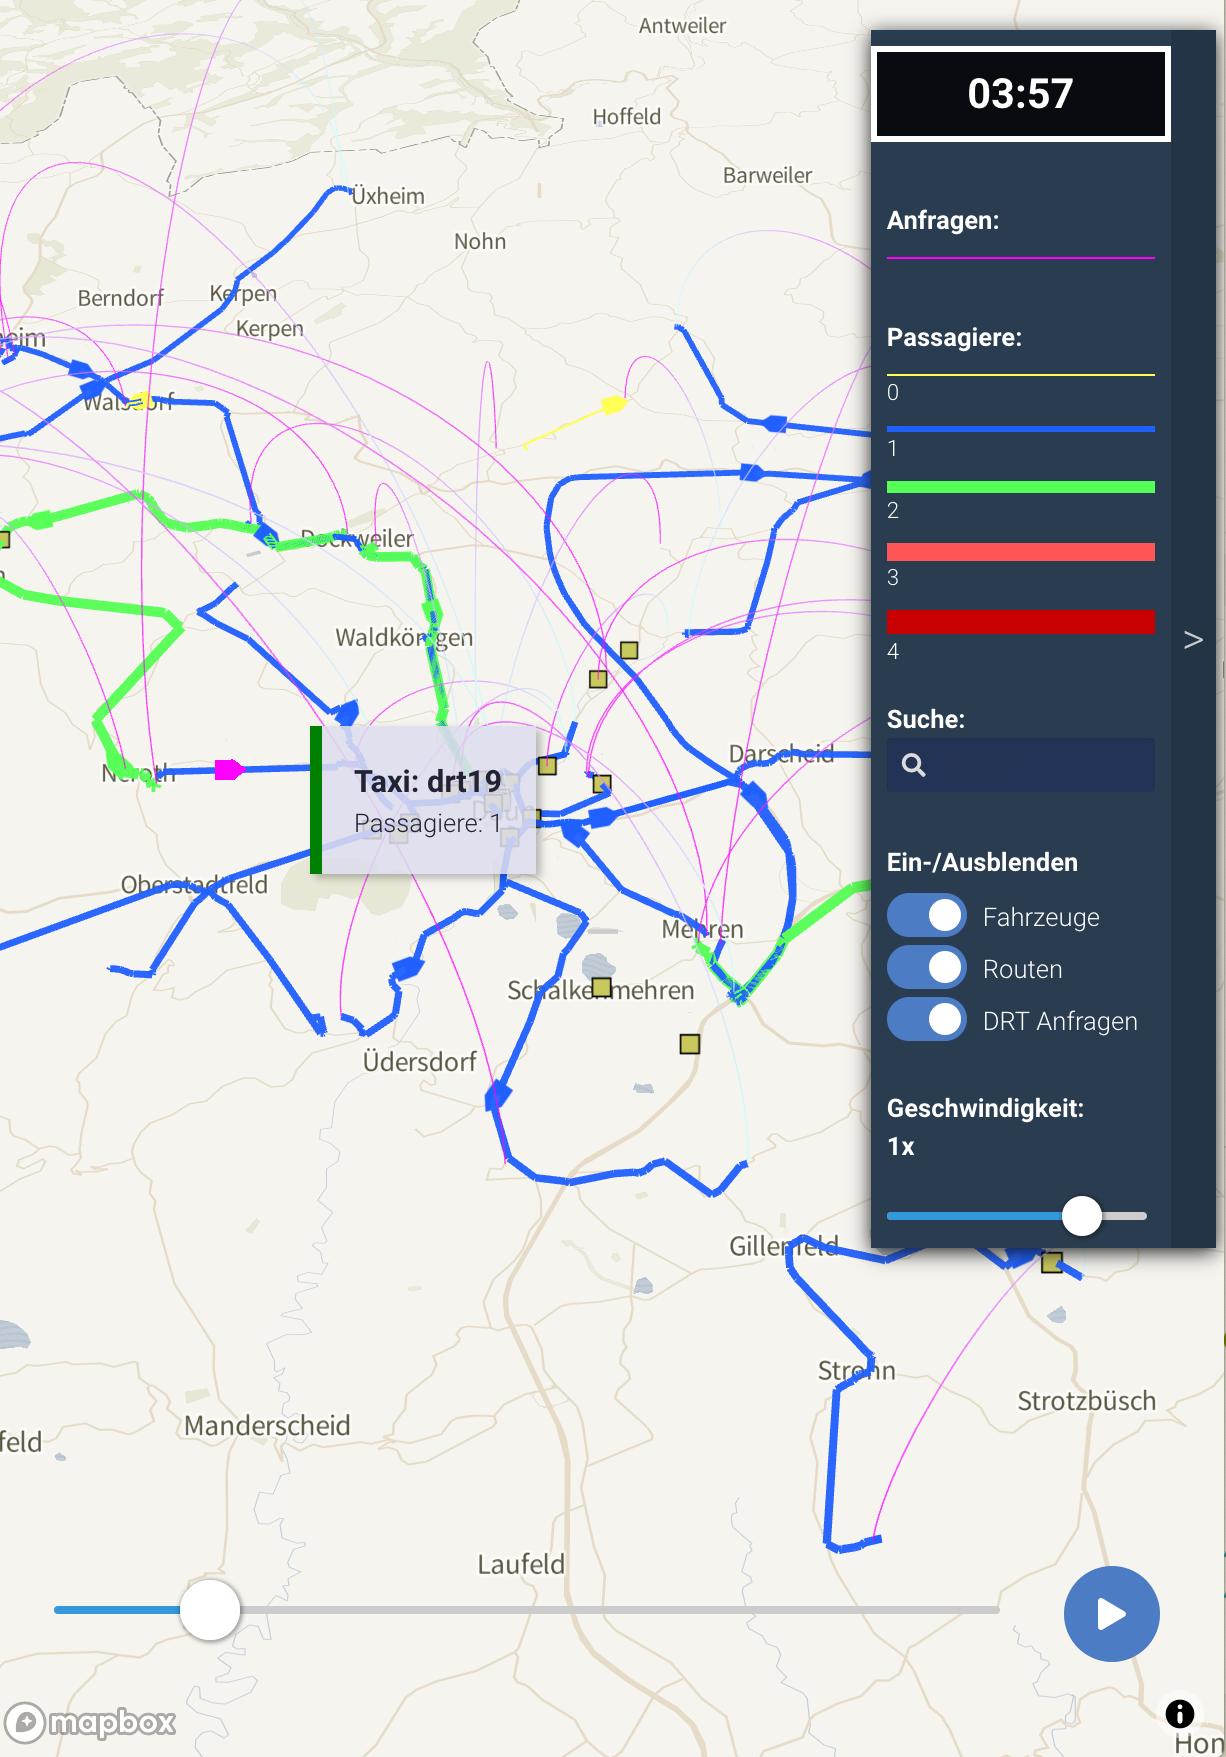
\includegraphics[width=\linewidth]{chapters/04-avov-pave/images/fig-drt-vehicles.png.pdf}
   \caption{DRT vehicles and routes}
   \label{fig:vehicles}
\end{minipage}
\begin{minipage}[c]{0.4\textwidth}
   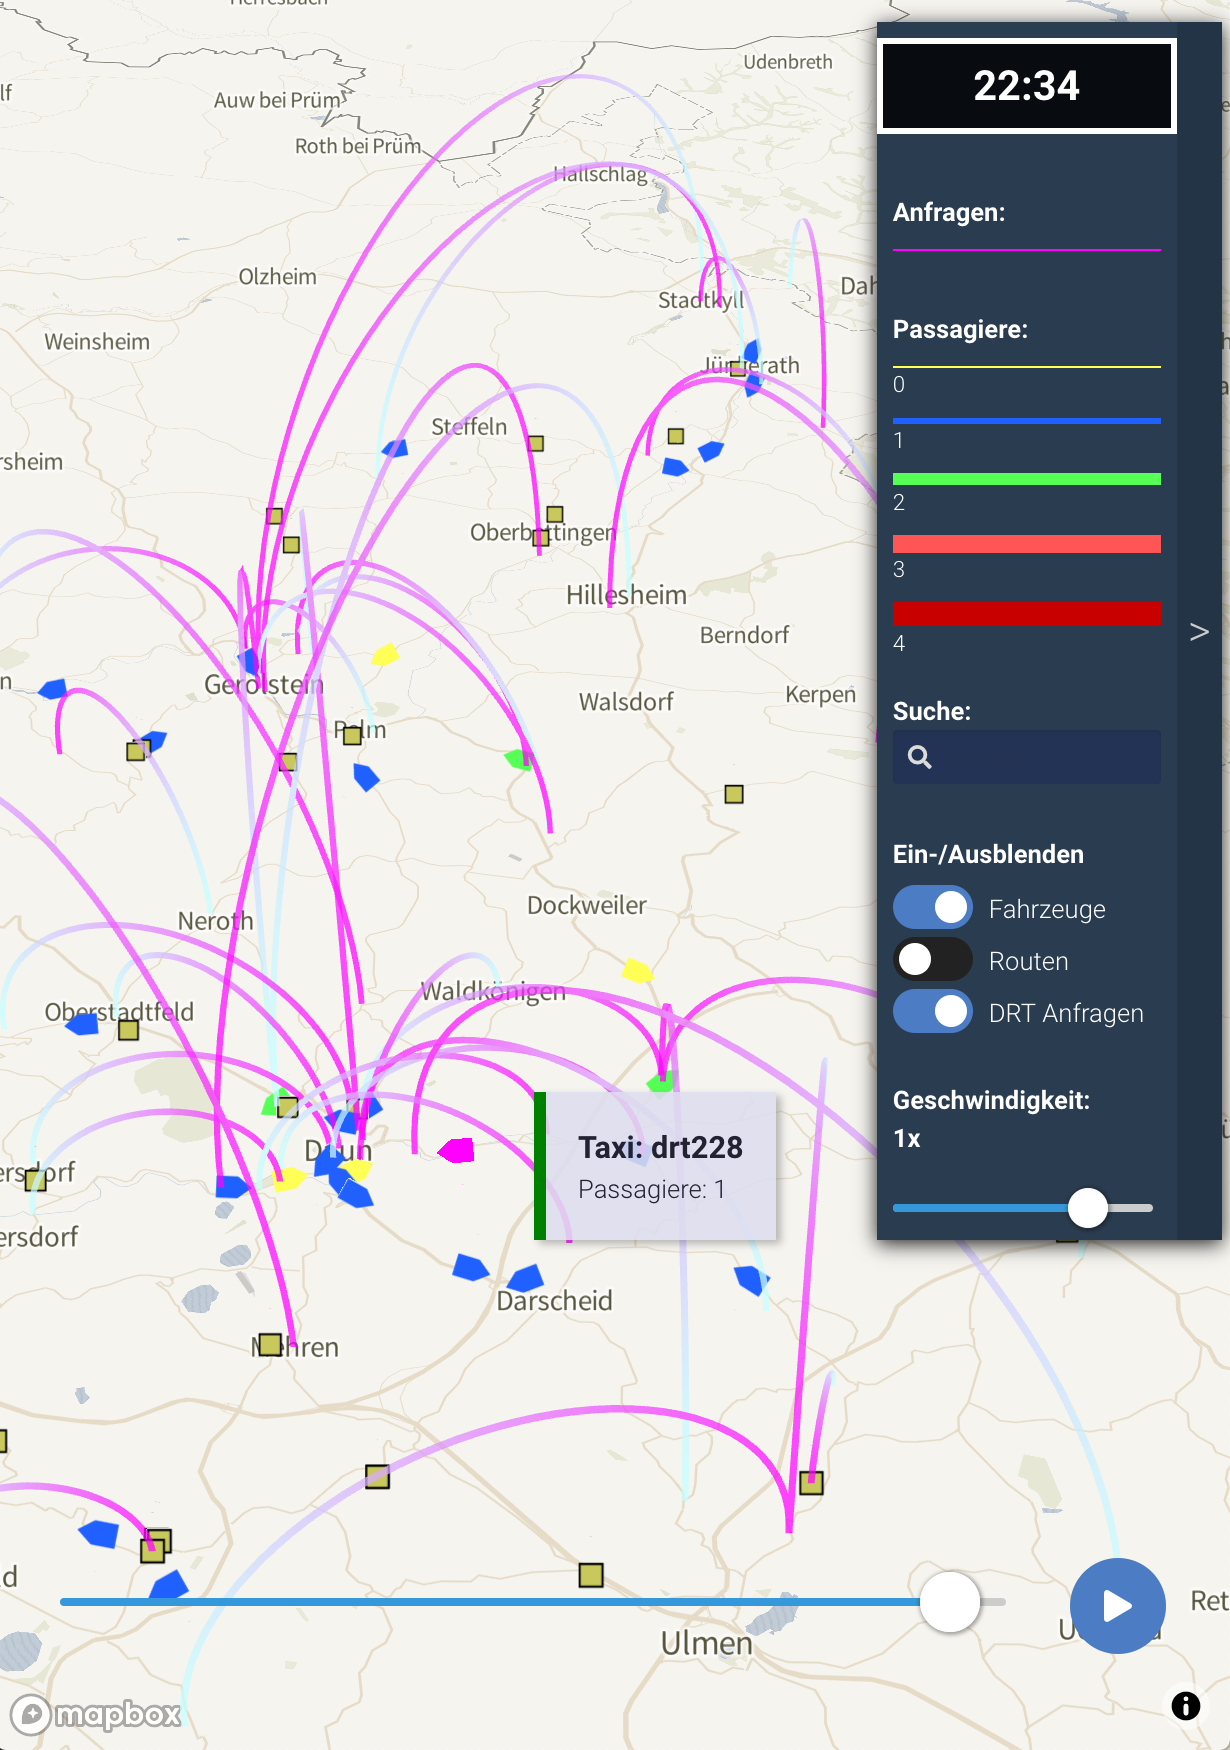
\includegraphics[width=\linewidth]{chapters/04-avov-pave/images/fig-drt-flyovers.png.pdf}
   \caption{DRT passenger origins and destinations}
   \label{fig:flyover}
\end{minipage}
\caption{Dynamic Response Transit (DRT) animation screenshots}
\end{figure}

\subsection{DRT Passenger and Vehicle volumes}

Aggregate summaries of roadway volumes depict total DRT pasenger or vehicle volumes in the entire simulation, or for specific times of day. The user can click on a specific link to see the diurnal (time of day) distribution of trips for that link, or can modify the time window being displayed for all links from total to a specific range, such as 6 A.M. to 9 A.M. if morning commute trips are being studied.

Difference plots compare the DRT scenarios to the "base case" depicting current conditions.

\begin{figure}[ht]
  \centering
  \begin{minipage}[c]{0.32\textwidth}
     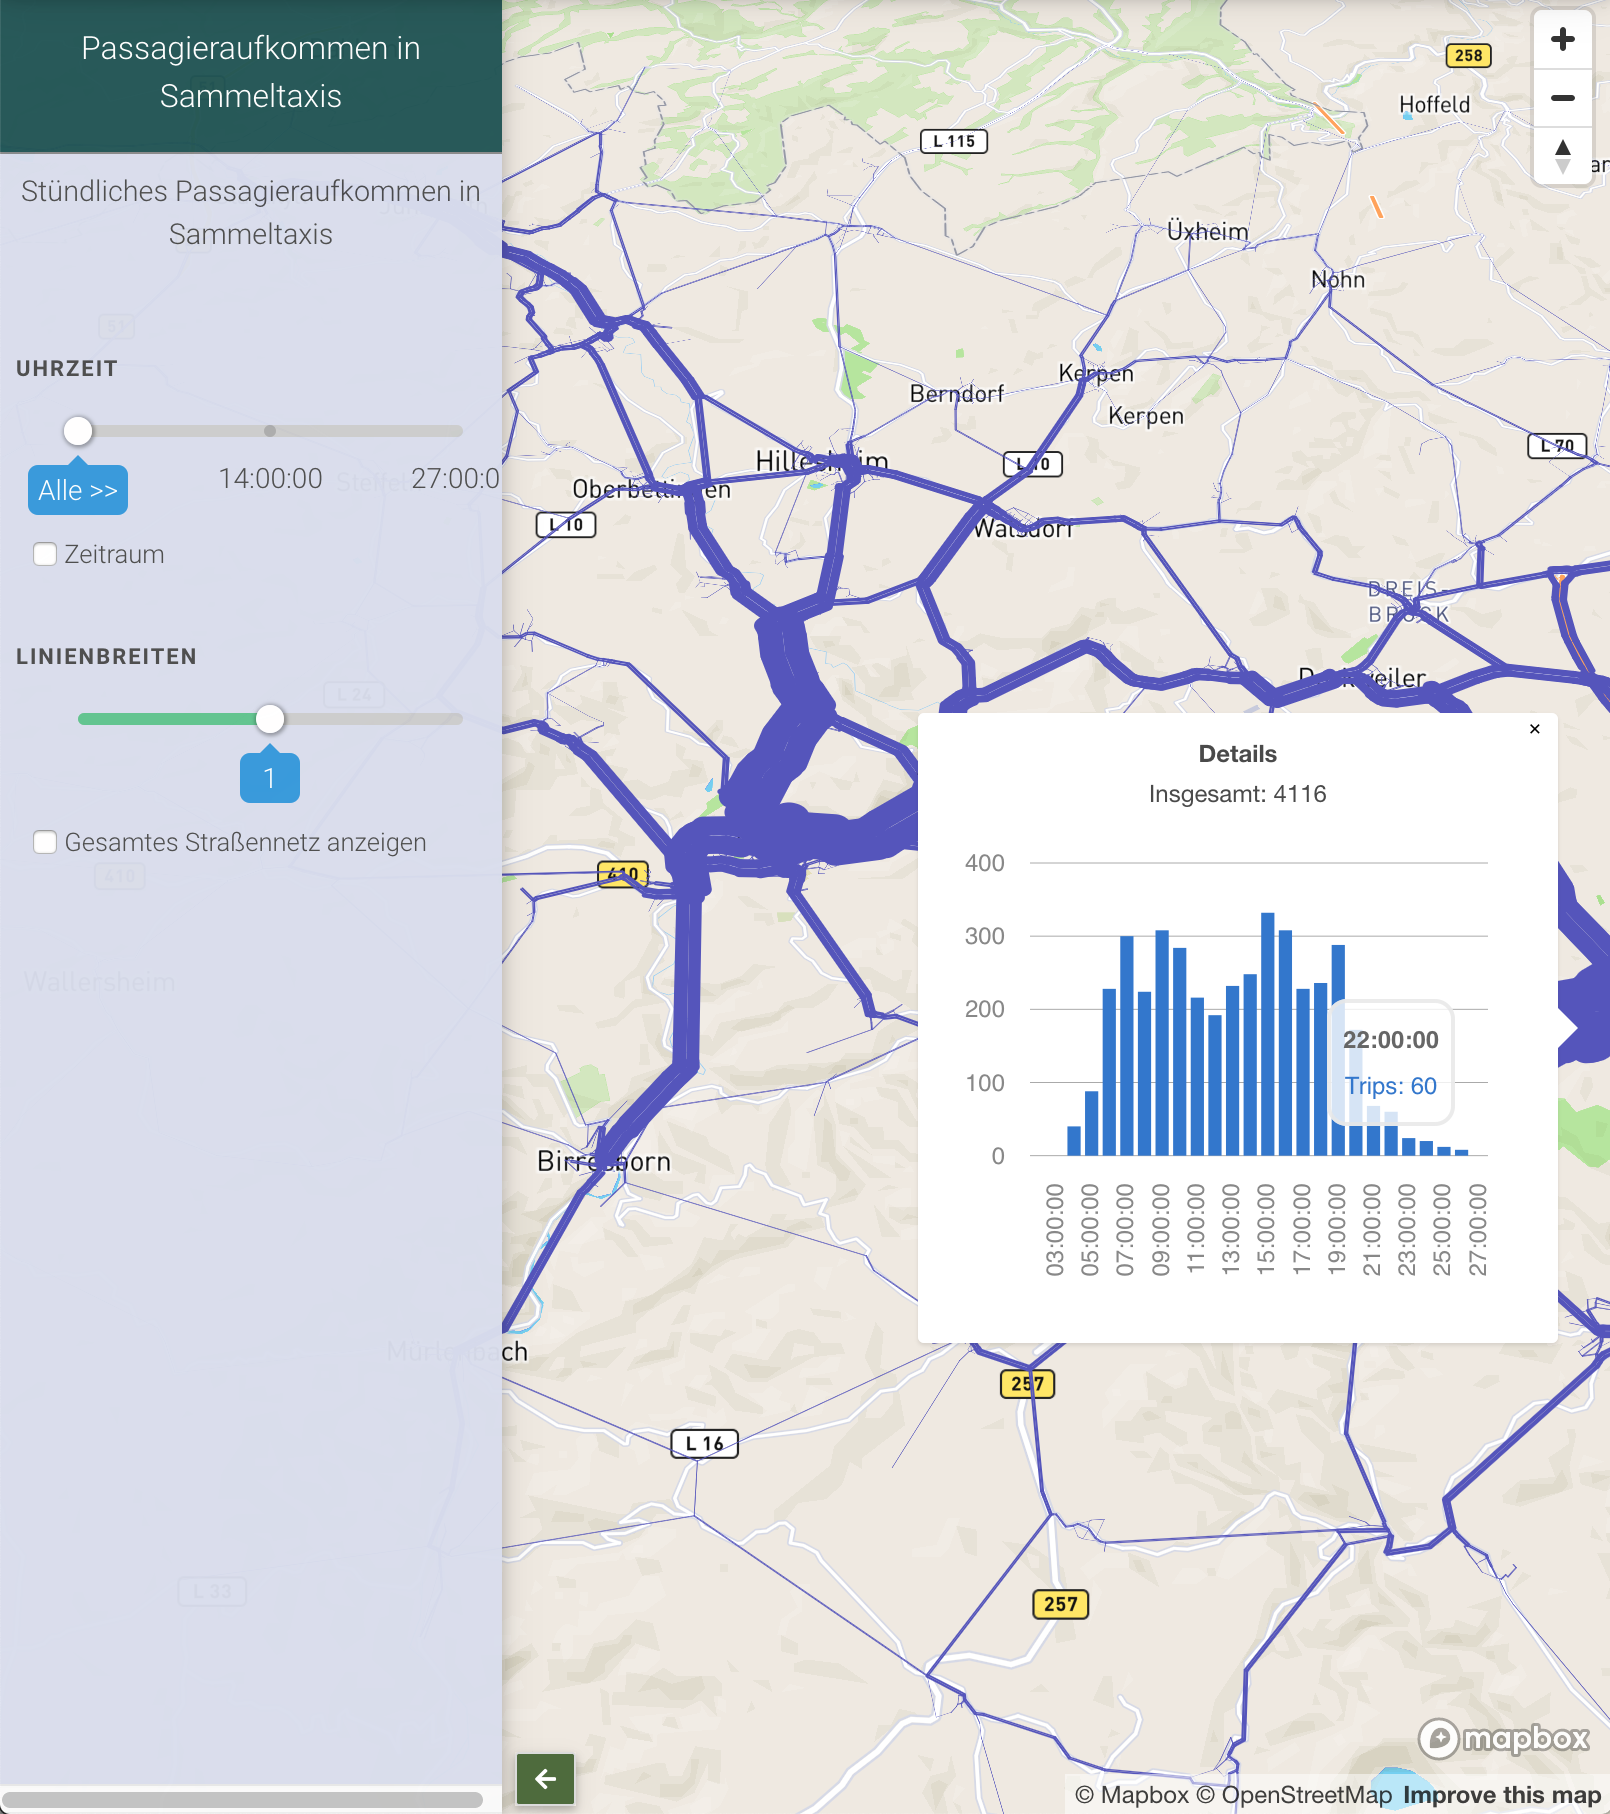
\includegraphics[width=\linewidth]{chapters/04-avov-pave/images/fig-link-vols.png.pdf}
     \caption{DRT Vehicle volumes, daily aggregation }
     \label{fig:vehicles}
  \end{minipage}
  \begin{minipage}[c]{0.32\textwidth}
     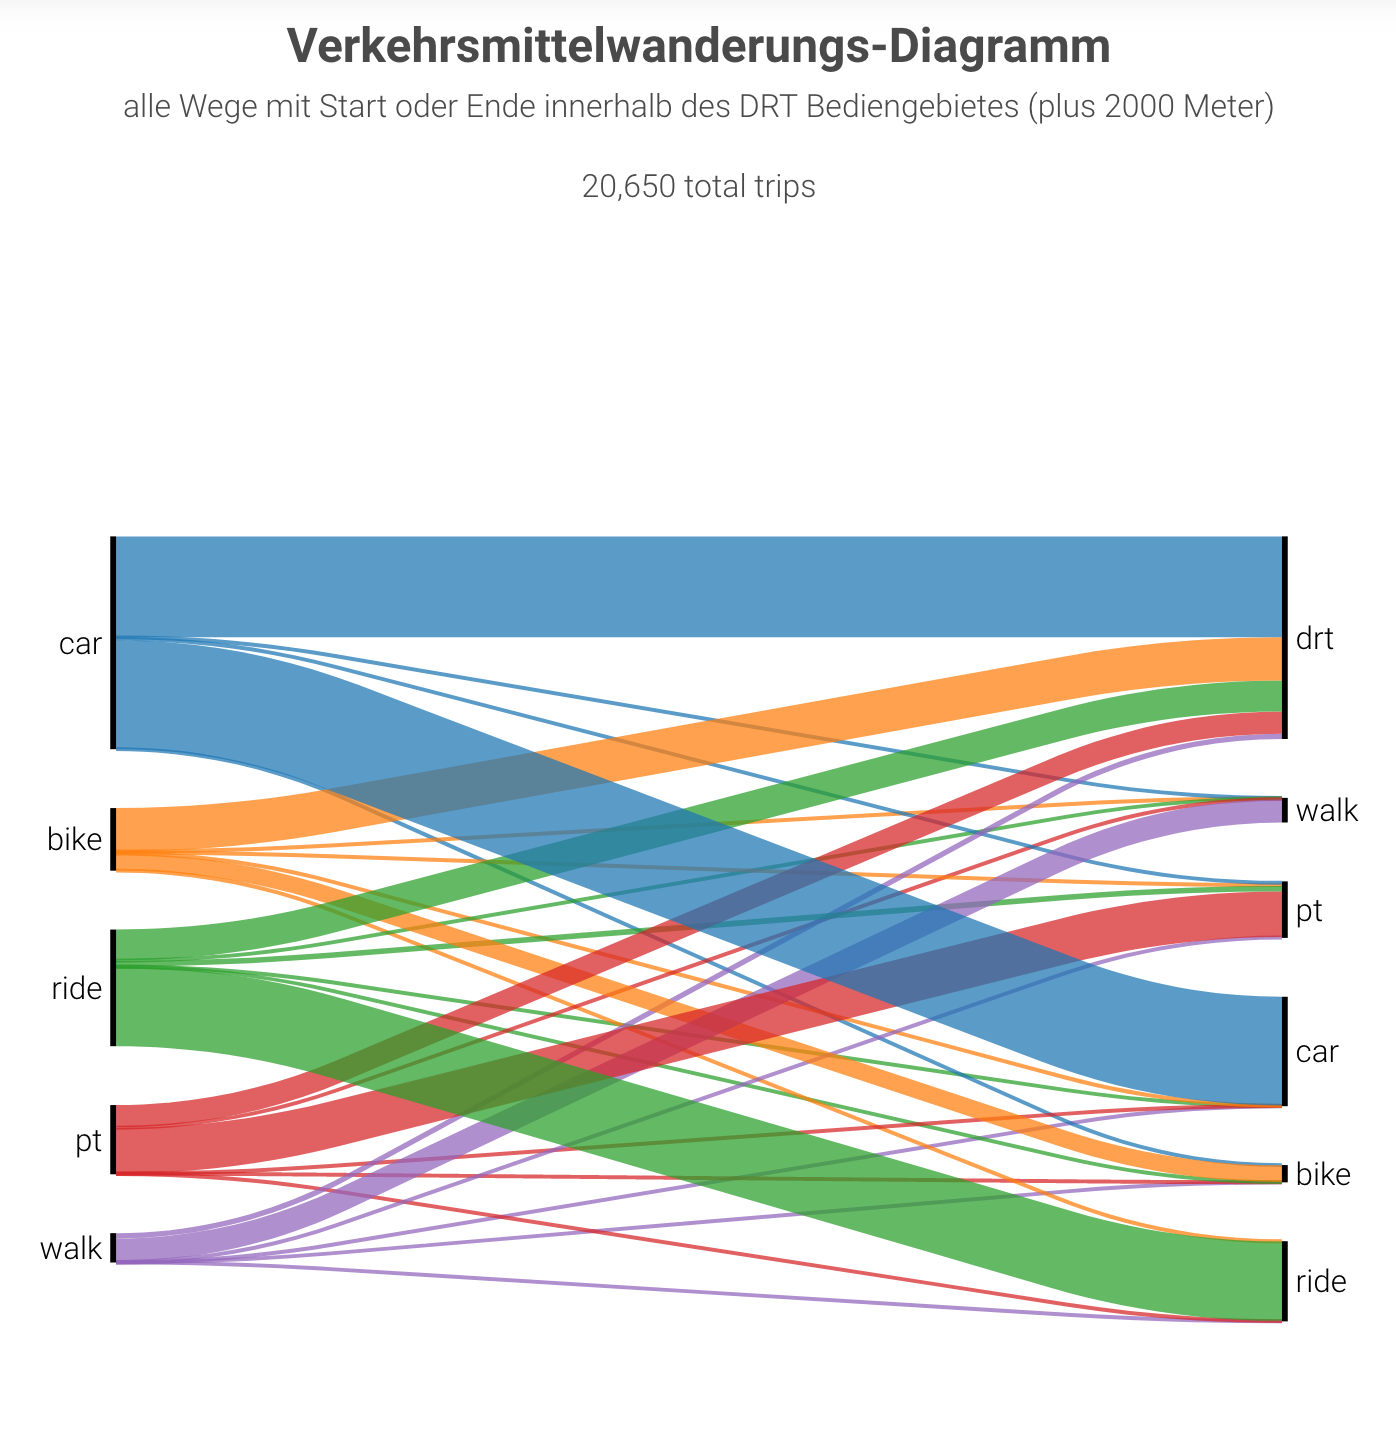
\includegraphics[width=\linewidth]{chapters/04-avov-pave/images/fig-mode-share.png.pdf}
     \caption{Mode shift, example DRT alternative vs. base case}
     \label{fig:flyover}
  \end{minipage}
  \caption{Dynamic Response Transit (DRT) further visualization examples}
\end{figure}


\subsection{Cross-Scenario Modal Shifts}

Users can also \emph{compare} the aggregate total mode shift from one scenario to another, in this study comparing DRT scenarios to the base case. These visualizations really highlight the degree to which the new DRT mode is "stealing" trips from existing transit and bicycle modes versus from private vehicles.


%% ----- RESULTS -----
\section{Results}
\label{results}

Throughout summer 2020, our team iterated on dozens of DRT scenarios: varying pricing structures, presence of drivers vs. fully automated service, service coverage areas, maximum wait time goals, and so on. In August 2020 we began the first public meetings with transit agency staff, with the fully operational website at \href{https://avoev-vsp.github.io}{avoev-vsp.github.io} (available in German only).

The final site displays a front page listing the results for 6-8 scenarios in each region, covering a wide spectrum of DRT scenarios. Then for each scenario, visualizations include the individual agent animations (see above) with occupancy, origin/destination, and routing details; mode shift summaries vs. base case; vehicle volume, passenger volume, and volume differences on roadway links compared to base case; aggregate levels of tripmaking for trips originating or destined to geographical areas ("hexagon plots"); as well as detailed model output summary graphs depicting general taxi occupancy levels by time of day and more.

Each outreach meeting started with technical staff describing the study, the agent-based model, and the results for each alternative in overview; followed by small break-out groups online, in which people could explore the scenarios and discuss the findings amongs themselves; and finally a return en banc for group discussion. No problems with bugs or site performance were reported.

Some direct feedback from analysts included:

\small{

\begin{displayquote}\emph{
  The DRT viz helped us understand better how the drt code works and find some issues, e.g. when the system is congested weird things can happen and a large group of vehicles with one passenger per vehicle only moves from the same start to the same destination at the same time (in an attempt to save each passenger a few seconds it serves them separately and wastes vehicles which then are missing for the next requests). It is really nice to have requests and vehicle occupancy shown, Via did only the latter after some pre-processing.
}\end{displayquote}

\begin{displayquote}\emph{
  The website obviously made the AVÖV workshops easier. Instead of only sharing our screen we could hand out a website where people could click themselves. Unfortunately it seemed that those listeners did not use the website a lot and rather kept listening to us. Some hypotheses: Maybe because sometimes a group of people shared one computer and their internet connection was bad, maybe because they are not used to that kind of interaction...
}\end{displayquote}

\begin{displayquote}\emph{
  The other plots like passengers/link or vehicles/link are not entirely new; some used QGis to produce those. However, the website forced us to actually produce all those plots systematically instead of 'we could do that plot, but maybe it's not necessary, let's look into something else or raw data only to avoid the hassle of setting up QGis...'
}\end{displayquote}

}

The feedback that some of these visualizations are not entirely "new" is expected: tools such as QGis and Via provide some very nice visualization capabilities already. They are not online tools, however, and are not accessible to non-technical staff such as at a public outreach meeting.

Given this level of feedback, we are pleased with the initial roll-out of the visualization platform, and expect to continue developing it for further analysis of dynamic-response transit systems.

%% ----- CONCLUSIONS -----
\section{Conclusions and Outlook}
\label{conclusions}

Several years of trial and error led us to this specific combination of technologies and techniques. The research team is deeply indebted to the developers of so many components and libraries on which this is based, all of which are freely available online and without which this work would have been entirely impossible. The final product is more than parts merely cobbled together: a usable, useful tool for decision-making now exists, and the DRT-specific extensions serve as a template for further work.

Paraphrasing Dennis Ritchie's early description of the UNIX system in \citet{Ritchie1978}, "Success lies not so much in new inventions but rather in the full exploitation of a carefully selected set of fertile ideas, and especially in showing that they can be keys to the implementation of a small yet powerful system."

Our successful experience using the platform in a public outreach setting confirms our belief that advanced agent-based simulations can be part of a decision framework and public policy discussions -- ultimately leading to better informed decision-making.

Further enhancements to the underlying platform and to the DRT visualization capabilities are ongoing; the plugin architecture enables other Javascript developers to write plugins for their own agent-based models and their own use cases, if they so desire.

The website remains online at \href{https://avoev-vsp.github.io}{avoev-vsp.github.io}. All code is available at \href{https://github.com/avoev-vsp/avoev-vsp.github.io}{github.com/avoev-vsp} and is licensed under the GNU GPL Version 3 \cite{FSF2007GnuGPL}. The authors welcome feedback and code contributions.

\section{Acknowledgements}
This research benefited from many discussions with Professor Kai Nagel, and was funded in part by the German Federal Ministry of Transport and Digital Infrastructure (funding number 16AVF2160)


\chapter{SimWrapper}
\label{ch:simwrapper}
% ------------------------------------------------------------------------------------
% # Chapter: SimWrapper
% ------------------------------------------------------------------------------------

Having confirmed the utility and capabilities of a fully browser-based
data visualization approach for three individual project portals, we
then set out to generalize the method. An entirely generic data
visualization platform is inherently more difficult than a project
portal, as every researcher investigates widely disparate questions and
will be focusing on completely different outputs. Where one researcher
may be using MATSim to predict future dynamic-response shared taxi
vehicle flows, another is doing emergency-response evacuation planning,
or emissions reduction through increased transit ridership efforts. The
tool needs to be extremely flexible.

% \begin{figure}
%   \centering
% 	\begin{minipage}{.75\textwidth}
% 		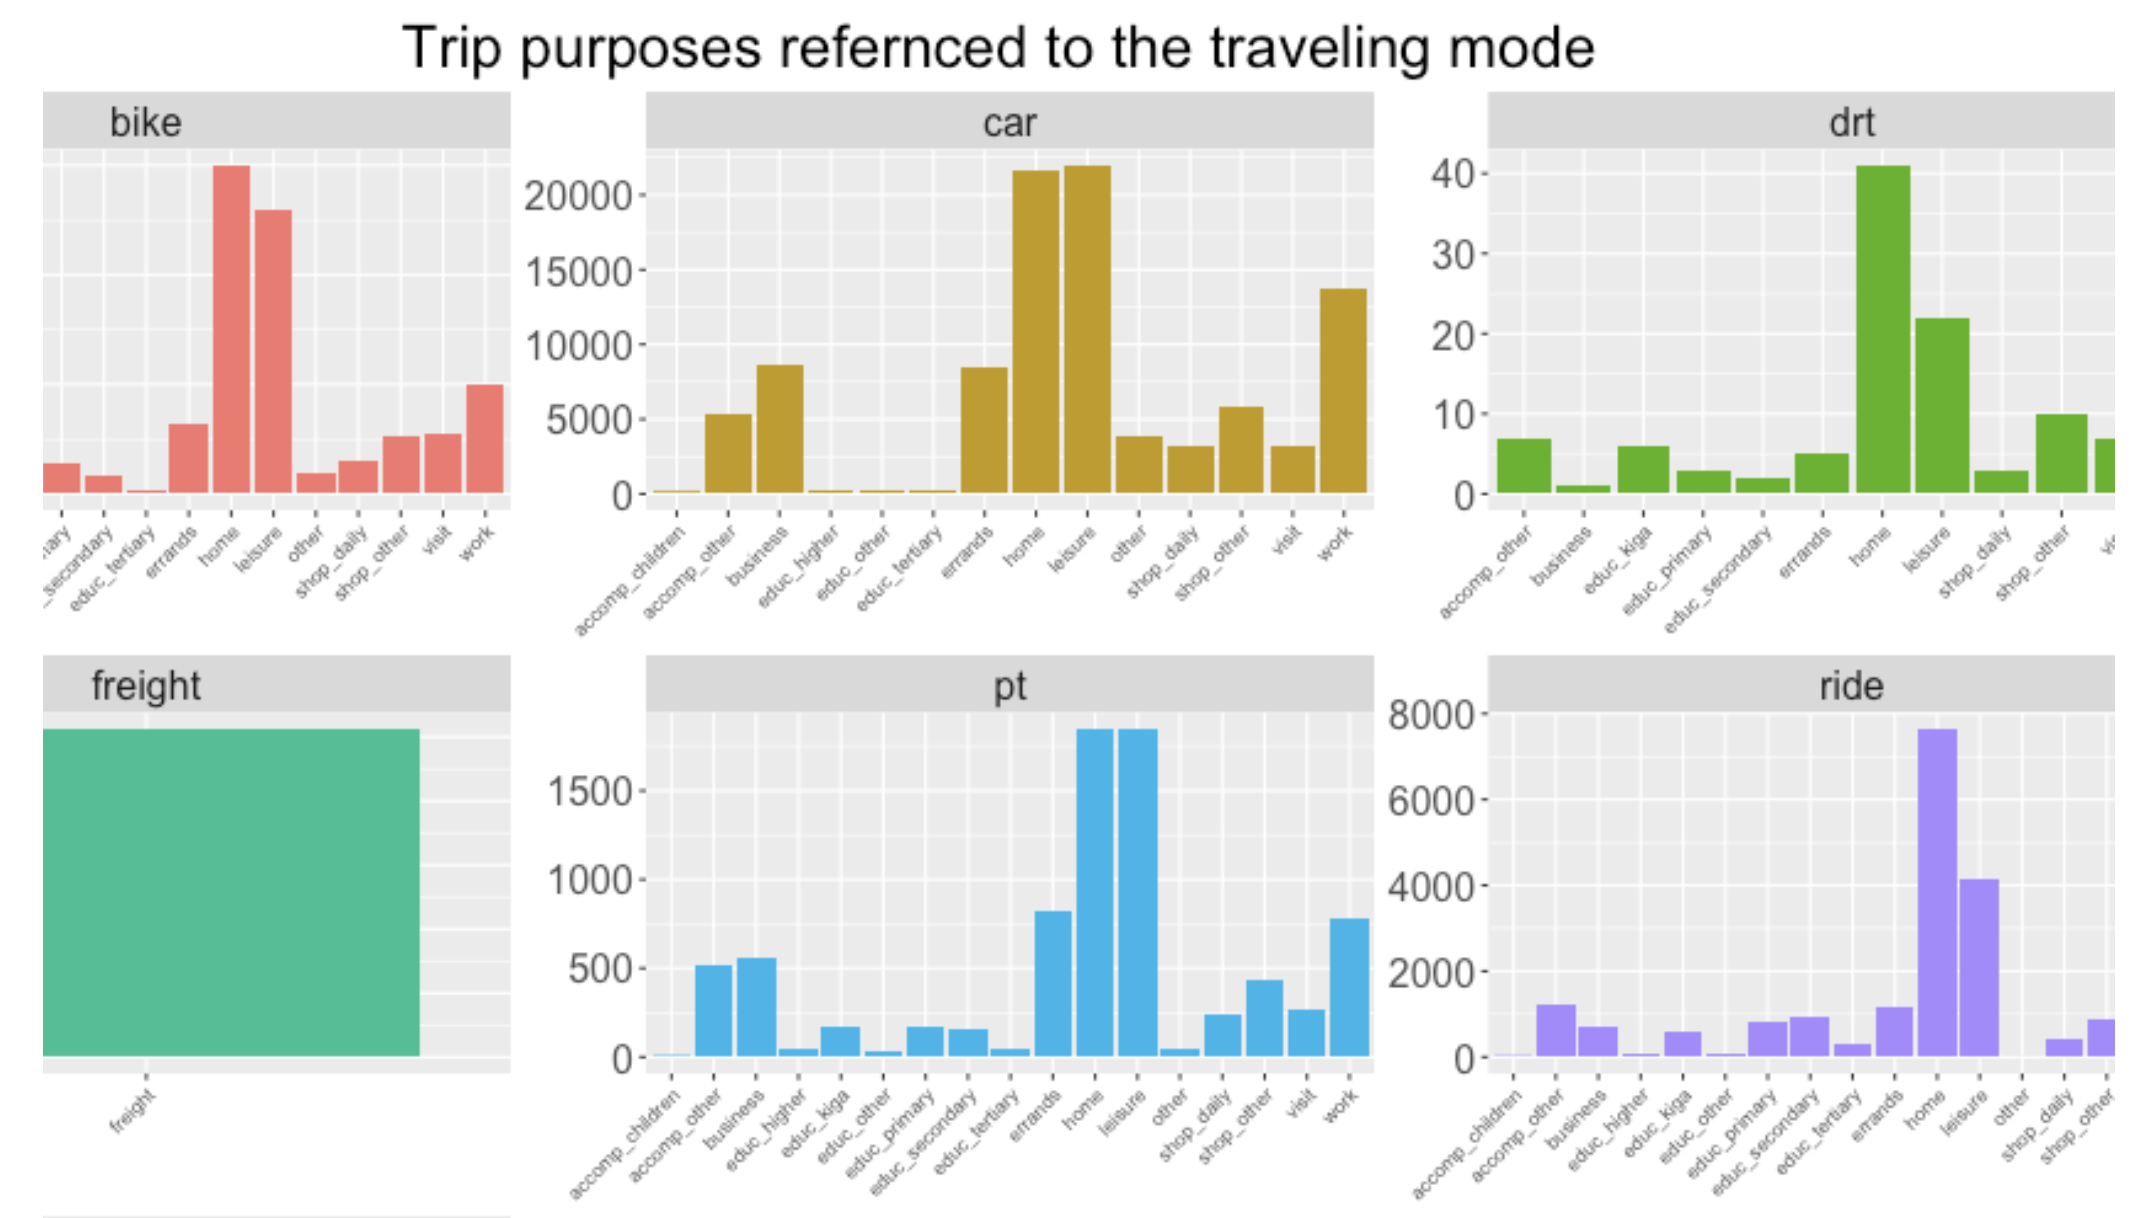
\includegraphics[width=\textwidth]{chapters/06-simwrapper/images/charts.png.pdf}
% 		\caption{CHart: stuff.}
% 		\label{fig:chartychart}
% 	\end{minipage}
% \end{figure}

This chapter describes \textbf{SimWrapper}, an open-source web-based
data visualization platform we developed with the goal that it be useful
for anyone working with MATSim outputs or even outputs from other
data-intensive microsimulation models.

% ------------------------------------------------------------------------------------
% ## SimWrapper in a Nutshell
% ------------------------------------------------------------------------------------

\hypertarget{overview-simwrapper-in-a-nutshell}{%
\section{Overview: SimWrapper, in a
nutshell}\label{overview-simwrapper-in-a-nutshell}}

Many design questions were already settled in the aforementioned
research YY.

SimWrapper, in a nutshell:

\begin{itemize}
\item
  \begin{enumerate}
  \def\labelenumi{(\arabic{enumi})}
  \item
    is a static website that runs client-side javascript in the form of
    a ``single page application'', a common approach in current web
    development that is compatible with all modern web browsers;
  \end{enumerate}
\item
  \begin{enumerate}
  \def\labelenumi{(\arabic{enumi})}
  \setcounter{enumi}{1}
  \item
    supports network-based file storage for public- and/or
    group-accessible shared data files (model runs), but has no other
    back-end server requirements and can run completely locally if no
    network file storage is available or needed;
  \end{enumerate}
\item
  \begin{enumerate}
  \def\labelenumi{(\arabic{enumi})}
  \setcounter{enumi}{2}
  \item
    allows the user to navigate through their local filesystem or shared
    network storage of model runs to view results that are saved in a
    specific folder, rather than a database-centric approach. This
    matches the design of MATSim and other simulation models which
    produce collections of output files by default;
  \end{enumerate}
\item
  \begin{enumerate}
  \def\labelenumi{(\arabic{enumi})}
  \setcounter{enumi}{3}
  \item
    provides a collection of data visualization archetypes that are each
    appropriate for displaying a certain type of data, for example
    various statistical chart types (bars, lines, area, pie), geographic
    data viewers supporting road and transit network link data, area
    aggregation (``choropleth'' and ``spider'') maps, XY coordinate
    plots, and many more;
  \end{enumerate}
\item
  \begin{enumerate}
  \def\labelenumi{(\arabic{enumi})}
  \setcounter{enumi}{4}
  \item
    can combine all of these disparate components into cohesive
    dashboards that the user can lay out in a flexible manner, using
    small declarative configuration files. These configurations can be
    applied across multiple projects or simulation runs;
  \end{enumerate}
\item
  \begin{enumerate}
  \def\labelenumi{(\arabic{enumi})}
  \setcounter{enumi}{5}
  \item
    is GDPR (General Data Protection Requirement) compliant by default,
    due to the complete lack of any user tracking, data uploads,
    servers, advertising, or any other privacy-compromising misfeatures.
    SimWrapper is not a product for sale; it is an open research
    platform, and can therefore forego these modern nuisances.
  \end{enumerate}
\end{itemize}

The following sections explore the design of SimWrapper in more detail.

\textbf{YY diagram of design}

% ------------------------------------------------------------------------------------
% ## Reusing existing components from previous projects
% ------------------------------------------------------------------------------------

\hypertarget{reuse-of-existing-framework-and-components}{%
\section{Reuse of existing framework and
components}\label{reuse-of-existing-framework-and-components}}

The starting point for SimWrapper was the PAVE project website described
in section YY. This ``single page application'' approach involves
selecting a curated set of javascript infrastructure libraries for
common needs, and then writing bespoke code for our specific use case
and the ``glue'' between the components.

Our experience with PAVE led us to select existing Javascript libraries
for the following:

\begin{itemize}
\item
  User interface interaction: the ``Vue'' framework YY is the primary
  glue that links the page layout with user interactions such as mouse
  clicks, running code when user-initiated events occur
\item
  Data loading: Most MATSim outputs are either tabular text files in CSV
  format, or compressed XML files with explicit schemas. The Papaparse
  and Fast-XML-Parser libraries handle loading these two data formats
\item
  Charting: the PAVE site included statistical charts such as bar, line,
  pie, and scatter plots, and used the Plotly javascript library. Plotly
  is very easy to use but not as feature-rich as some other choices; see
  below YY for updated capabilities
\item
  Geographic data on maps: our initial efforts using the Mapbox
  javascript library led us to the more performant Deck.gl collection of
  map-based visualizations.
\item
  Animation: Three.js is a very flexible 3D animation library that is
  used for PAVE vehicle animation visualizations.
\end{itemize}

All of these libraries share compatible open-source licenses, and are
included in SimWrapper under the terms of those licenses.

% ------------------------------------------------------------------------------------
% ## Modifications needed for a generic tool
% ------------------------------------------------------------------------------------

\hypertarget{modifications-necessary}{%
\section{Modifications necessary}\label{modifications-necessary}}

Direct user feedback, described in detail in section YY, allowed us to
map out a set of changes and improvements for the generic tool. In
summary, changes were needed in the following categories:

\begin{itemize}
\item
  Performance. The network link viewer in particular was slow to load
  datasets for large simulations. This was not a problem for PAVE or
  AVÖV because the study areas were less populated.
\item
  Flexibility. Each of the data visualization components needed to be
  made much more flexible. For example, the PAVE link viewer assumed
  that input data was specified by time period, whereas a generic tool
  needs to depict any sort of data.
\item
  Output traversal. While PAVE had a hard-coded set of alternatives that
  could be browsed in a simple manner, a generic tool needs some sort of
  model run traversal capability; a way to browse the hierarchical file
  storage available.
\item
  Stability and resilience. The PAVE site included almost no error
  message reporting or helpful debugging infrastructure, because expert
  analysts carefully crafted the inputs for each alternative. A generic
  tool needs to be tolerant of user mistakes and helpful in guiding the
  user when inputs are lost or malformed.
\item
  Better defaults plus configurability. We do not intend to replicate a
  full-featured desktop application, of which there are many in the
  Geographic Information System (GIS) realm. Rather, users expressed a
  desire for a set of clear, curated defaults that have some
  configurability. For much more advanced configuration, a
  professionally-developed package such as QGis is likely more
  appropriate.
\end{itemize}

\hypertarget{audience}{%
\subsubsection{Audience}\label{audience}}

The PAVE website was intended to be public-facing: both agency staff and
actual members of the public could navigate the site. It presented a
small set of YY six alternatives, depicting the same visualizations for
each alternative.

SimWrapper could be public facing, but is predominantly used in its
current form by researchers and professional analysts at public
agencies.

YY

% ------------------------------------------------------------------------------------
% ## Accessing files via a Web Browser
% ------------------------------------------------------------------------------------

\hypertarget{accessing-files-through-a-web-browser}{%
\section{Accessing files through a web
browser}\label{accessing-files-through-a-web-browser}}

The use case of file storage via departmental file server is
well-explored and very functional, as expressed in the project websites
for AVÖV, PAVE, and COVID-Sim.

A key difference between the earlier project websites and SimWrapper is
the need to ``meet the users where they are'' -- in other words, we
cannot rely on there being a departmental file server with a public API
endpoint serving data files. One of the primary feedback elements from
the initial MatHub implementation described in chapter YY was that it
was too onerous to upload model run outputs to a second server system
before being able to view or analyze anything. In addition to being
wasteful of space (and MATSim outputs can be gigabytes in size!), it is
time-consuming.

For regular users in the middle of their research workflow, something
else is needed. Most of our internal users run simulations either on
their personal laptop/desktop machines, or on the university compute
cluster, which has extensive attached storage but no public-facing
access via the web. Furthermore, these runs are often not intended to be
immediately publicized.

Thus we explore several avenues for enabling users to view their
outputs, described here.

% ------------------------------------------------------------------------------------
% ### How SimWrapper access files via HTTP
% ------------------------------------------------------------------------------------

\hypertarget{how-simwrapper-access-files-via-http}{%
\subsection{How SimWrapper access files via
HTTP}\label{how-simwrapper-access-files-via-http}}

SimWrapper is designed to allow browsing of files from
administrator-defined HTTP URLs, which represent the root of the file
storage for that project. For example, the PAVE project datasets are all
stored on the VSP public file server at the URL

\url{https://svn.vsp.tu-berlin.de/repos/public-svn/matsim/scenarios/countries/de/berlin/projects/pave/website/}

That URL is the defined ``root'' of the project; all of the project
dashboard configurations, model outputs, and processed data files exist
in various subfolders below that location. The PAVE website at
https://vsp.berlin/pave is set up to read files from that base URL. (But
refer to section YY for a discussion of CORS configuration, which is
necessary to allow one website to read the files stored on another.

SimWrapper elevates this to allow multiple configured root filesystems;
the public VSP file server is one such root, but others can also be
configured and are displayed on the home page of SimWrapper. Each root
is expected to provide HTTP directory access to this storage: SimWrapper
needs to be able to \emph{view directory listings} and \emph{retrieve
file contents}. SimWrapper never writes any files anywhere; it is
read-only.

% ------------------------------------------------------------------------------------
% ### Local files
% ------------------------------------------------------------------------------------

\hypertarget{local-files-on-a-personal-laptopdesktop}{%
\subsection{Local files on a personal
laptop/desktop}\label{local-files-on-a-personal-laptopdesktop}}

This design presents a problem for local files: By design, all web
browsers explicitly forbid file-system access from any websites by
default. This default is certainly a good default; no one wants any
random website to start sniffing around their home directory.

But in our case this is not any random website: we \emph{want}
SimWrapper to see the files in some of our local folders. How can this
be accomplished?.

After several explorations including raw HTML files opened directly,
arcane experimental browser flags (always vendor specific!), and other
less fruitful avenues, the one method that consistently works for all
browsers is as follows: for browsing local files on a machine, first
start up a small helper application which is itself a simple HTTP
server. This tiny server responds to HTTP requests and delivers the
directory contents requested. The server listens on ``localhost'',
i.e.~your own computer, generally on port 8000. So the full URL is
\url{http://localhost:8000/}.

Once this is set up and running, this HTTP endpoint can be accessed in
SimWrapper just like any other external file storage. SimWrapper knows
be default to look for files at URL \url{http://localhost:8000}.

As part of this research we wrote a very small Python library which
provides this server. Any machine with Python 3.x installed can run
\texttt{pip\ install\ simwrapper} to install this mini file server, and
then run it by navigating to their data folder and running the command
\texttt{simwrapper\ serve}. That includes all of the server components
and configuration needed to server files to SimWrapper.

Some configuration notes:

\begin{itemize}
\item
  The local HTTP server will only serve the files from inside the
  working directory in which it is started, including any subfolders. No
  other folders on the user's machine are exposed.
\item
  The computer's operating machine has default firewall and router rules
  that will generally prohibit any outside access from other computers
  on the LAN or the Internet. This can be modified; see YY
\item
  Some configuration details for the server that are important for our
  use case: we must enable access from websites at different URLs using
  ``CORS'' configuration headers; see YY
\item
  Some browsers (Safari, and now recent builds of Chrome) sometimes
  block access to localhost sites or http sites (vs.~https sites), see
  discussion at YY
\item
  Every language framework already includes some sort of ``Tiny HTTP
  Server'' library for just these types of uses: in Python it is in the
  \texttt{http.server} library, in Java there is the Jibble
  SimpleWebServer. Our \texttt{simwrapper} python tool leverages the
  existing Python infrastructure.
\item
  We also wrote a java version, published as
  \texttt{mini-file-server.jar} for users who are more comfortable
  running Java-based software than Python.
\end{itemize}

The Python tool including source and user documentation is currently
available at \url{https://pypi.org/project/simwrapper/}.

The Java tool is currently available at
\url{https://github.com/simwrapper/mini-file-server}

\hypertarget{data-security-and-privacy}{%
\subsubsection{Data security and
privacy}\label{data-security-and-privacy}}

With this setup, the SimWrapper site itself is loaded from the Internet,
but once loaded, the user's data never leaves their computer. SimWrapper
is an entirely client-based system with absolutely no upstream server.
The javascript runs in the users' browser, accessing files available on
localhost only -- also on the user's own computer. Nothing leaves the
browser. If there are privacy or confidentiality issues with model
outputs, SimWrapper can still be used for analysis in this ``localhost''
mode.

% ------------------------------------------------------------------------------------
% ### Files on Compute Cluster servers
% ------------------------------------------------------------------------------------

\hypertarget{files-residing-on-the-university-compute-cluster-accessed-via-ssh}{%
\subsection{Files residing on the university compute cluster, accessed
via
SSH}\label{files-residing-on-the-university-compute-cluster-accessed-via-ssh}}

This local-http-server paradigm can be extended to access files on any
remote university computer cluster using the SSH (``secure shell'')
protocol.

SSH is usually the protocol (and command) used to log into remote
systems. There is a parallel command which allows ``mounting'' the
remote file system using the SSH protocol. The remote files are mapped
to a folder on the user's system; once mounted, the user can browse the
files inside that folder as if they were local files (but generally more
slowly, depending on network throughput conditions).

\begin{itemize}
\item
  Linux users can install the command \texttt{sshfs} to add this
  capability;

  \begin{itemize}
  \item
    once installed, a command similar to
    \texttt{sshfs\ username@cluster.math.tu-berlin.de:/net/myfiles\ cluster}
    will mount the remote folder \texttt{/net/myfiles} to my local
    folder \texttt{cluster}. You would change the username, URL, and
    folder names to match your situation.
  \item
    \texttt{sudo\ umount\ cluster} or similar to unmount.
  \end{itemize}
\item
  YY MacOS is similar to Linux but requires installing the sshfs fuse
  driver first
\item
  YY Windows users have many options for FUSE-based sshfs support, this
  repo is nice one \url{https://github.com/billziss-gh/sshfs-win}
\end{itemize}

% ------------------------------------------------------------------------------------
% ### Files on other machines: simwrapper here
% ------------------------------------------------------------------------------------

\hypertarget{files-residing-on-another-machine-on-the-local-lan-network}{%
\subsection{Files residing on another machine on the local LAN
network}\label{files-residing-on-another-machine-on-the-local-lan-network}}

A challenging use case presented by users is one or more central
``modeling server'' machines on the local LAN, where most runs are
performed and which contain the simulation outputs.

The aforementioned localhost-based HTTP server does not work in this
situation, because a user sitting at their computer, opening the
Internet-based SimWrapper website, trying to read files served via
localhost on the modeling server, will always be blocked by browser
security measures. After many hours trying to find a way to sneak around
these restrictions, we accepted that this security measure is working as
designed, and we need a different approach.

The reason this approach is blocked is because the SimWrapper website is
hosted on a secure ``HTTPS'' server, while the localhost files must be
served without encryption using HTTP. Setting up an encryption
certificate is difficult because internal LAN machines don't typically
have world-findable DNS entries. This combination of secure and insecure
content is blocked by all browsers.

A workaround is to serve the files and the site from the same file
server, instead of using the Internet-based SimWrapper that is hosted at
vsp.berlin. We are already asking users to run a small file server to
access their local files, thus extending that file server to also serve
the necessary javascript and HTML is a natural extension.

And this is what we have done: a special mode is added to the
\texttt{simwrapper} python tool named \texttt{simwrapper\ here}. Now the
little server will serve both the file contents of the folder in which
it is started, \emph{and} the SimWrapper website itself.

The user runs \texttt{simwrapper\ here} on the file server instead of
\texttt{simwrapper\ serve}, \emph{noting the full URL printed in the
console}, and then on their personal computer browses to that URL
instead of to vsp.berlin/simwrapper. In this manner, the site and any
local files stored on that server are made available, together.

This also implies that SimWrapper can be used completely offline once it
is installed.

% ------------------------------------------------------------------------------------
% ### Special case: Google Chrome
% ------------------------------------------------------------------------------------

\hypertarget{special-case-chrome-and-the-file-system-access-api}{%
\subsection{Special case: Chrome and the ``File System Access
API''}\label{special-case-chrome-and-the-file-system-access-api}}

Google Chrome and a subset of other browsers based on the Chromium
codebase implement an experimental API known as ``File System Access
API''. This is not part of the official Web specification, and it may
never be adopted by other browser vendors.

But for users running Google Chrome, this experimental API provides
another avenue for accessing local files, one which completely
eliminates the need for the local file server approaches above.

This is considered ``progressive enhancement,'' or in other words,
adding features to the website when the browser is identified as
supporting them.

On Chrome, users will see an additional element on the main page of
SimWrapper, a button allowing them to grant access to local files. The
browser will open a standard folder-picking dialog followed by a warning
that granting this permission will allow the SimWrapper site to view the
files in that folder. Et Voíla, that is exactly what we need.

Once permission is granted, local files are immediately visible without
any additional configuration. This permission can be revoked and may be
re-requested every time the browser restarts.

YY show browser grant access dialog

% ------------------------------------------------------------------------------------
% ## Converting purpose-built vizes into Generic Data Viewers
% ------------------------------------------------------------------------------------

\hypertarget{converting-purpose-built-visualizations-into-generic-data-viewers}{%
\section{Converting purpose-built visualizations into generic data
viewers}\label{converting-purpose-built-visualizations-into-generic-data-viewers}}

The underlying infrastructure -- the build system, the user interaction
libraries, and the choice of off-the-shelf components -- was more or
less complete after the PAVE, AVÖV, and COVID-Sim projects were
operational. But the specific views needed a great deal of retooling to
make them useful in a generic manner.

This section describes some of the most challenging aspects of this
process of genericizing SimWrapper.

% ------------------------------------------------------------------------------------
% ### Link Viewer
% ------------------------------------------------------------------------------------

\hypertarget{link-viewer}{%
\subsection{Link viewer}\label{link-viewer}}

The link viewer was originally scoped to display link volumes only, such
as a typical ``bandwidth plot'' commonly used in travel modeling. Even
for PAVE this was short-sighted, as the project team quickly found other
uses for the viewer such as link-based emissions.

Two critical updates made for SimWrapper are (1) the removal of the
assumption that the data inputs will always have time period data in the
columns, plus a summary ``grand total'' column; and (2) that colors and
widths must be configurable, preferably separately.

These changes are now part of SimWrapper -- see YY for a typical plot.

YY show a bandwidth plot

User testing shows that a great deal more is still necessary to meet
user expectations. Data filters and configurable hovers are two of the
most-requested enhancements.

YY user testing

% ------------------------------------------------------------------------------------
% ### XY Data Plots
% ------------------------------------------------------------------------------------

\hypertarget{xy-hexagon-plots}{%
\subsection{XY Hexagon plots}\label{xy-hexagon-plots}}

Much data is not link-based, even for transport simulations. Activity locations, home locations, pickups and dropoffs for transit and taxi modes, all have geographic coordinates associated with them but are not necessarily attached to specific links.

A new visualization type, the ``XY Hexagons'' plot, depicts these types of data by aggregating them into user-definable hexagonal buckets. The number of points inside the hexagons corresponds to a color or height; this is user-configurable.

YY show XY Hexagon plot

The default MATSim output \texttt{output\_trips.csv} includes this type of data, and is automatically viewable without any configuration at all if it is present in a SimWrapper data folder.

% ------------------------------------------------------------------------------------
% ## Calculation Tables
% ------------------------------------------------------------------------------------

\hypertarget{calculation-tables}{%
\section{Calculation tables: providing top-line summary metrics}\label{calculation-tables}}

Early in the development of SimWrapper, user feedback identified the need for reporting basic summary statistics and generating common aggregate values from model runs. These top-level summaries provide the first indication of useful results, such as overall mode share, average travel times, total emissions, and so forth. In addition, these measures are an excellent way to "sanity-check" a model run; in other words, to identify any obvious glaring errors in those topline numbers when compared to previously-established norms.

The first element needed is a straightforward way for users to specify the inputs, outputs, and formatting of calculation tables, compatible with the file-based configuration approaches already in use for the graphical visualizations. A second challenge is to formulate a clear and accurate scheme for specifying the needed calculations, including statistical transformations of the inputs such as counts, sums, and so on. Finally, the tool must perform those calculations in memory and produce the display the results.

These three elements are explored in order.

% ------------------------------------------------------------------------------------
% ### Calculation Table Config: Inputs, Files, Outputs
% ------------------------------------------------------------------------------------

\hypertarget{calculation-tables-definition}{%
\subsection{Specifying calculation table files, inputs, and outputs }\label{calculation-tables-definition}}

The most robust way to generate and display a table of numbers is by having the user develop their own post-processing scripts which output a simple CSV with the summary values and labels that they need. For this approach, nothing special is needed; whatever data analysis pipelines the analyst is already using are sufficient. Especially for more complex post-processing needs, using a high-quality platform such as Python or R is the recommended path.

For more simple summaries, we develop a way to extract and minimally process typical MATSim data files including CSV and XML formats. This is based on experience with the hesitancy of some analysts in our department to write Python and R scripts (since they are far more familiar with Java programming). If all one needs is the sum of a column of values or the count of some event types, learning Python and debugging a Python script is perhaps overkill.

As the file-based YAML configuration paradigm for SimWrapper is at this point well-established, a new YAML configuration schema for table calculations is the most natural way to express these table definitions.

A new \texttt{table-*.yml} YAML schema containing four sections emerged from extensive iteration with users. The four required sections are:

\begin{itemize}

  \item \textbf{files}: The set of input file or files required for the table. These can be raw MATSim outputs or the results of any pre- or post-processing that has already occurred in the analyst data pipeline.

  \item \textbf{interactive input entries}: This is a list of end-user-editable entries that are visible on interactive web form. Some calculations benefit from having a variable input which the user can specify; imagine fuel cost per liter, or number of vehicles in a taxi fleet. Each of these entries can have a default value.

  \item \textbf{calculations}: An ordered list of mathematical calculations to be performed. Variables, data columns, and interactive elements specified above are combined in equations as needed. This is described in more detail below.

  \item \textbf{outputs}: The final table entries are specified with formatting and labels.

\end{itemize}

Three of the four sections --- \emph{files}, \emph{interactive entries}, and \emph{outputs} --- are trivially specified and do not require extensive exposition here: they are straightforward definitions of file names, titles, and formatting directives. These are well-documented in the YY documentation available on the SimWrapper Website (\cite{SimWrapperWebsite}).

The calculations are explored next.

% ------------------------------------------------------------------------------------
% ### Calculation Table DSL: Specifying the Equations
% ------------------------------------------------------------------------------------
\hypertarget{calculation-tables-dsl}{%
\subsection{Specifying calculations using a Domain-Specific Language}\label{calculation-tables-dsl}}

The final and most important piece of specifying calculations is devising the equation format to be used in the YAML configuration, which brings together the interactive value inputs, the required input files, data columns in those files (and any data manipulations thereon), and combines them all in understandable algebraic equations that can be solved by the tool.

This is more akin to a "domain-specific language" (DSL) YY ACRONYM than a configuration file.

\cite{Visser2008} defines a domain-specific language as follows, "A domain-specific language (DSL) is a high-level software implementation language that supports concepts and abstractions that are related to a particular (application) domain." Visser explains further that a DSL is in essence "the encapsulation of design and implementation knowledge from a particular application or technical domain. The commonalities of the domain are implemented directly in a conventional programming language or indirectly in code generation templates, while the variability is configurable by the application developer through some configuration interface."

This is precisely what the YAML calculation definitions set out to do: allow a user who is an expert in the dataset and the needed transformations for a particular metric, to define that in a manner that doesn't require them to write a data analysis script in a full-fledged programming language such as R or Python.

YY continue



% - Need a way to write equations
% - How to specify pieces of data from the inputs: files, columns, elements
% - transformations
% - filtering: two ways


% ------------------------------------------------------------------------------------
% ### Calculation Tables: Map/Reduce your way to an answer
% ------------------------------------------------------------------------------------
\hypertarget{calculation-tables-map-reduce}{%
\subsection{Calculating summary values via "map/reduce"}\label{calculation-tables-map-reduce}}

% - solve each equation, in top-down order
% - map/reduce columns of data using statistical functions
% - substitute values from out data
% - nerdamer does the math
% - final values can be displayed according to the formatting rules in 'output'


YY Show PAVE example run output with Sankey, numbers, etc

% ------------------------------------------------------------------------------------
% ## Dashboards
% ------------------------------------------------------------------------------------

\hypertarget{dashboards-combining-visualizations-to-support-decisionmaking}{%
\section{Dashboards: combining visualizations to support
decisionmaking}\label{dashboards-combining-visualizations-to-support-decisionmaking}}

A dashboard is a page laid out with multiple charts, plots, and
visualizations all together. The layout is defined in a YAML file that
contains the types of plots and their configuration parameters, all in
one place.

YY SHOW Dashboard \emph{Dashboards usually show several at-a-glance
summary metrics.}

In SimWrapper, a folder containing any number of \texttt{dashboard-*}
YAML files will display the dashboards in addition to the usual folder
browser view. When multiple dashboard YAML files exist, they will be
shown as multiple navigation tabs on the page.

\begin{itemize}
\item
  The layout consists of a set of named \textbf{rows}. The row name
  themselves are not shown anywhere, they are there to help organize the
  file.
\item
  Each \texttt{row} consists of a list of chart objects. By default, all
  objects in the row will be laid out horizontally from left to right,
  in equal widths. This can be configured.
\item
  Finally, each element in a row has specific properties that define the
  actual chart or visualization that will be displayed.

  \begin{itemize}
  \item
    \textbf{type} The chart or plot type, e.g.~\texttt{pie},
    \texttt{bar}, \texttt{flowmap}, etc. See the individual chart docs
    for all available plots.
  \item
    \textbf{title} The name of the plot
  \item
    \textbf{description} A brief description (optional)
  \item
    \textbf{width} One can set \emph{relative widths} by adding the
    \texttt{width:\ {[}number{]}} property. Charts have a default width
    of 1. Thus in a row with 3 charts, if the width of the first object
    is 2, then {[}2+1+1{]} means the first object fills 50\% of the row,
    and the remaining two objects fill 25\% each. (optional)
  \item
    \textbf{props} The set of configuration settings for this chart,
    such as the dataset to load, which columns to use, etc.
  \item
    \emph{The chart type determines the set of valid properties!}
  \end{itemize}
\end{itemize}

This system of defining dashboards in configuration has been used to
great effect in many internal studies

YY Show Düsseldorf (Hamburg?) ?

% ------------------------------------------------------------------------------------
% ## Project sites: Re-using and organizing outputs
% ------------------------------------------------------------------------------------

\hypertarget{project-traversal-and-organizing-outputs}{%
\section{Project traversal and organizing
outputs}\label{project-traversal-and-organizing-outputs}}

Project organization for MATSim is left up to the user: there is no
central database or general organizing principle which analysts must
adhere to. Thus different teams will find different ways to store their
data: by project, by date, by scenario type, etcetera. Some may use a
very flat structure with a defined naming scheme, while others will use
deeply nested folders to keep things tidy.

Because of this flexibility in MATSim, SimWrapper needs to be able to
handle deeply hierarchical storage as well as extremely large folders
full of runs.

There is much more room for improvement here, but the basic format of a
file and directory browser, which allows the user to ``drill down'' into
subfolders, will be part of any solution.

% ------------------------------------------------------------------------------------
% ### Calculation Table DSL: The Calculation Engline
% ------------------------------------------------------------------------------------


\hypertarget{project-level-configuration}{%
\subsection{Project-level
configuration}\label{project-level-configuration}}

Users often expressed interest in setting up standardized output
summaries in the form of dashboards, specific link- or xy-data
comparison plots, etc., and to use those for every model run for that
project.

This is addressed by having a \texttt{simwrapper} folder in or above the
output-data folders. The simwrapper folder contains any common
configuration files, whether they be dashboard layouts, individual
visualization parameters, or table calculation definitions. See YY for
more details on the configuration of individual components.

% ------------------------------------------------------------------------------------
% ## User Feedback and Iteration
% ------------------------------------------------------------------------------------

\hypertarget{user-feedback-and-iteration}{%
\section{User feedback and
iteration}\label{simwrapper-user-feedback}}

% ------------------------------------------------------------------------------------
% ## Limitations
% ------------------------------------------------------------------------------------

\hypertarget{limitations}{%
\section{Limitations}\label{simwrapper-limitations}}

% ------------------------------------------------------------------------------------
% ## Discussion
% ------------------------------------------------------------------------------------

\hypertarget{discussion}{%
\section{Discussion}\label{simwrapper-discussion}}


% \chapter{Commercial Transport}
% \label{ch:wirtschaftsverkehr:ch}
% % !TeX spellcheck = en_US
% !TEX root = ../../phd.tex

\todo[inline]{WIV schreiben}

In diesem Kapitel sollen zunächst die grundlegendne Zusammenhänge und Besonderheiten des Wirtschaftsverkehrs beschrieben werden.... 

\section{Überblick}
\label{gl-wiv-Überblick:sec}


\section{Güterverkehr als Teil des Wirtschaftsverkehrs}
\label{gl-wiv-Güterverkehr:sec}


\section{Logistiknetzwerke}
\label{gl-wiv-Logistik:sec}

%%%%%%%%%%%%%%%%%%%%%%%%%%%%
%%%%%%%%%%%%%%%%%%%%%%%%%%%%


% \chapter{Emissions}
% \label{ch:emissionen:}
% % !TeX spellcheck = en_US
% !TEX root = ../../phd.tex

\todo[inline]{Schadstoffe schreiben}

In diesem Kapitel werden einige wesentliche Informationen zu Scahdstoffen und ihren Wirkungen gegeben.

\section{Überblick}
\label{gl-schadstoffe-Überblick:sec}

%%%%%%%%%%%%%%%%%%%%%%%%%%%%
%%%%%%%%%%%%%%%%%%%%%%%%%%%%

\section{Schadstoffe im Verkehr}
\label{gl-schadstoffe-Verkehr:sec}

%%%%%%%%%%%%%%%%%%%%%%%%%%%%

\subsection{exhaust}
\label{gl-schadstoffe-Verkehr-sec:exhaust}

%%%%%%%%%%%%%%%%%%%%%%%%%%%%

\subsection{non-exhaust}
\label{gl-schadstoffe-Verkehr-sec-non-exhaust}

%%%%%%%%%%%%%%%%%%%%%%%%%%%%
%%%%%%%%%%%%%%%%%%%%%%%%%%%%

\section[HBEFA]{HBEFA: Handbook of ....}
\label{gl-schadstoffe-HBEFA:sec}

%%%%%%%%%%%%%%%%%%%%%%%%%%%%
%%%%%%%%%%%%%%%%%%%%%%%%%%%%


% \chapter{Modeling and Simulation}
% \label{ch:modellierung-simulation}
% % !TeX spellcheck = en_US
% !TEX root = ../../phd.tex

\todo[inline]{Modellierung und Simulation}
This chapter is dedicated to the modeling and simulation of (freight) traffic. This includes a general introduction to agent-based models (\cref{sec:gl-modsim-MATSim}). In the introduction of the software \acrshort{MATSim}, and some of its extensions which are used in this thesis are presented. 
This chapter concludes with a presentation of tour planning using the tour planning software \gls{jsprit} (\cref{sec:gl-modsim-vrp-jsprit}).


\section{Agent-based Modeling and Simulation}
\label{sec:gl-modsim-ABM}

\todo[inline]{abm schreiben}artinst
Agenten-basierte Modelle sind....

%%%%%%%%%%%%%%%%%%%%%%%%%%%%
%%%%%%%%%%%%%%%%%%%%%%%%%%%%

\section{The Multi-Agent Transport Simulation Software MATSim}
\label{sec:gl-modsim-MATSim}

\todo[inline]{MATSim-Teil selbst schreiben}


\subsection[MATSim]{MATSim}
\todo[inline]{anderen Namen finden für MATSim-main}
\rewrite{
The \acrfull{MATSim} is an open source software for agent-based transport simulation. It is an activity-based, extendable framework implemented in Java, which is designed for large-scale scenarios. In addition to a common base, several optional extensions 
are available (see \url{https://matsim.org/extensions}) \citep{MATSimBook}.
\gls{MATSim} is based on a co-evolutionary algorithm, where each iteration consists of the following three steps: Traffic simulation, scoring, and replanning. %(cf. Fig. \ref{fig:matsim}). 
\gls{MATSim} simulates agents -- normally persons -- and their daily plans, which consist of activities like home or work and trips between their activity locations. These plans are simulated and then scored based on their experienced performance. After the scoring some agents try to improve their plans, e.g. by selecting a different route or modifying activity start and end times. For this, several strategies are available to generate new or modified plans. After this replanning step, a new iteration of the simulation starts with the modified plans. After running the specified number of iterations, \gls{MATSim} terminates after the scoring step\citep{MATSimBook}
}


%%%%% TEXT von IK!!!!
%This \nameCref{simultaneous-sec:SimulationFramework} provides a brief overview of the activity-based transport simulation \gls{matsim}
%%\gls{matsim}%
%%%
%%\footnote{
%	%%
%	%Multi-Agent Transport Simulation, see www.matsim.org
%	%%
%	%}
%%
%which is used and extended in this thesis.
%\gls{matsim} is an open-source software developed under the terms of the GNU General Public License (\url{https://www.gnu.org/licenses/}), version 2 or later, published by the Free Software Foundation (\url{https://fsf.org}). The core code and several extensions are available on GitHub (\url{https://github.com/matsim-org/matsim}). The software structure follows a modular design which allows for an easy replacement or extension of the default functionality. The overview of \gls{matsim} provided in this \nameCref{simultaneous-sec:SimulationFramework} refers to the simulation setup which is most relevant for this thesis. The following is a combined and edited version of \gls{matsim} related descriptions in several articles that have been previously published, see, e.g., \citet{KaddouraNagel2016HeterogeneousVTTSPricing, KaddouraNagel2017CongestionPricing, KaddouraNagel2016CongestionNoiseOptimization, KaddouraKroegerNagel2015NoiseInternalization, Kaddoura2014CongestionPricingBerlin}, and \citet{NeumannEtAl2016MindTheGap, KaddouraEtAl2014AgentBasedPtOptimization} for the description related to \gls{pt}, or \citet{KaddouraEtAl2018SAVpricing} for the description related to \glspl{SAV}.
%
%In \gls{matsim}, each transport user is simulated as an individual agent. The agents' initial behavior has to be provided in the form of travel plans describing the daily activity patterns (e.g.,  home-work-shopping-home), the activity locations, the activity end times and information about the trips between these activities. The initial travel behavior is then modified applying an evolutionary iterative approach. In each iteration, (1) the travel plans are executed (Traffic simulation), (2) scored (Evaluation) and (3)~modified (Learning). (1) represents the agents' physical behavior; (2) and (3) describe the agents' mental behavior.
%
%\begin{enumerate}
%	\item \textbf{Traffic Simulation}
%	All travel plans are simultaneously executed and the transport users interact in the simulated physical environment. Traffic congestion and vehicle movements are simulated applying a queue model \citep{Gawron1998IterativeAlgorithmto}. Each road segment (link) is modeled as a \emph{First In First Out} queue with certain attributes, i.e, a free speed travel time $t_{free}$, a flow capacity $c_{flow}$ which limits the outflow \citep[in the literature often referred to as `bottleneck congestion', see, e.g.,][]{VanDenBerg2011Thesis}, and a storage capacity $c_{storage}$ which limits the number of vehicles on a link and causes spill-back. Each time step, typically 1~\gls{sec}, the state of each link's queue is updated. A vehicle is only moved from link $l_{1}$ to link $l_{2}$ if (i) the free speed travel time (given by the freespeed and length of link $l_{1}$) has passed, (ii) the inverse of the flow capacity has passed since the last vehicle left link $l_{1}$, and (iii) there is space on link $l_{2}$. Individual movements of agents can be aggregated to traffic flows that are found to be consistent with the fundamental diagram \citep[see, e.g.,][]{AgarwalEtcMixedTraffic}.
%	
%	\gls{matsim} also simulates the interaction of \textbf{\gls{pt}} users, transit vehicles and road traffic. The transit schedule provides all planned \gls{pt} operations. Transit vehicles may be delayed by (i) other road users and (ii) \gls{pt} users. Transit vehicles are included in the traffic flow simulation, thus, buses and cars may compete for the same limited road capacity. Each stop can be configured to either block the traffic or to allow overtaking whenever a bus stops. Depending on the vehicle type, i.e., the number of doors, and the assumption regarding simultaneous or sequential boarding/alighting, transit vehicles may be delayed by passengers at transit stops. In case a vehicle is fully loaded, additional boardings are denied and passengers will have to wait for the next transit vehicle.
%	Vehicles of one transit line can serve different tours. Consequently, the delay of one vehicle can be transferred to the following tour. In the case of a delay, the driver will try to follow the schedule by shortening dwell times (if no person wants to alight or board) as well as slack times.
%	For a detailed description of \gls{matsim}'s \gls{pt} dynamics, see \cite{Rieser2010} and \cite{Rieser2015PublicTransportMatsim}.
%	
%	The simulation of \textbf{\glspl{SAV}} is based on an existing module for dynamic vehicle routing problems \citep{Maciejewski2015DVRPInBook, MaciejewskiBischoffHoerlNagel2017DVRPTestbed} and an existing module for the simulation of taxis or \glspl{SAV} \citep{BischoffMaciejewski2016ANTAVBerlin}. \gls{SAV} users need to order an \gls{SAV} once they have left their activity location, wait for an available \gls{SAV} to arrive, get on the \gls{SAV} and get off the \gls{SAV} at the destination. \glspl{SAV} interact with each other and other vehicles, e.g., \glspl{CC}, and may get stuck in traffic.
%	
%	\item \textbf{Evaluation}
%	For each agent, the executed plan is evaluated based on agent-specific predefined behavioral parameters and utility functions. A plan's deterministic utility (often referred to as 'score') typically consists of two parts: (i) the generalized travel cost or trip-related disutility (e.g., travel time, monetary payments) and (ii) the utility gained from performing activities:
%	\begin{equation}
%		V_{p, i}= \sum_{a=1}^{A} \Big( 
%		%
%		V_{p,a}^{act} + V_{p,a}^{trip}
%		%
%		\Big) \ ,
%		\label{matsim-plan-utility}
%	\end{equation}
%	% 
%	where $V_{p,i}$ is the person $p$'s total utility (deterministic part) for a given plan $i$; $A$ is the total number of activities; $V_{p,a}^{act}$ is the
%	(positive) utility earned for performing activity $a$; and $V_{p,a}^{trip}$ is the (usually negative) utility earned for traveling to activity $a$. Activities are assumed to wrap around the 24-\acrshort{h}-period, that is,
%	the first and the last activity are stitched together. In consequence, there are as many trips between activities as there are activities. The first part typically considers the mode of transportation, the travel time, waiting, access and egress times and monetary costs (e.g., operation costs, fares, tolls).
%	The latter part is based on the approach by \cite{CharyparNagel2005ga4acts} where the marginal gain is typically positive but decreases with the duration spent at the activity location:
%	\begin{equation}
%		V_{p,a} = \beta^{perf}\cdot t^{typ}_{a} \cdot \ln\left( t^{perf}_{p,a} \middle/ t_{0,a} \right) \ ,
%		\label{matsim-eq:utilityPerf}
%	\end{equation}
%	% 
%	where $t^{perf}_{p,a}$ is the time person $p$ performs activity $a$, $t^{typ}_{a}$ is an activity's \emph{typical duration}, $\beta^{perf}$ is the marginal utility of performing an activity at its typical duration, and $t_{0,a}$ is defined as
%	\begin{equation}
%		t_{0,a} = t^{typ}_{a} \cdot \exp\left( -1 \right) \ ,
%		\label{decongestion-eq:t0}
%	\end{equation}
%	see \citet[][Sec.~97.4.2]{MATSimBook} for a discussion of this setting.
%	%a scale parameter 
%	%% \kai{Das stimmt vermutlich nicht mehr, oder?  (``uniform'' vs.\ ``relative'')}
%	%which is irrelevant as long as activities cannot be dropped.
%	%% \ihab{Auch bei 'relative' haben wir doch den $t_{0,a}$ parameter, und m.E. kann man den immer noch als 'scaling parameter' beschreiben. Ich hab jetzt einfach mal die Definition f\"ur $t_{0,a}$ hinzugef\"ugt. Das mit der priority spar ich mir hier mal, weil das an keiner Stelle relevant ist.}
%	Further activity-related constraints can easily be incorporated. An activity can only be performed during opening times. If an agent arrives at an activity location before or after the activity is open, the early or late arrival penalty results from the opportunity cost of time which is approximately equivalent to $\beta^{perf}$. Additionally, there may be a late arrival penalty $\beta^{late}$ which comes on top of the opportunity cost of time if an agent arrives after the \emph{latest arrival time} which can be specified for each activity.  Depending on the agent-specific travel plans, in particular the number and types of activities, agents are differently pressed for time, resulting in different \glspl{VTTS}.
%	%
%	
%	\item \textbf{Learning}
%	\label{introduction-sec:matsim-choice-dimensions}
%	For the majority of agents, the plan to be executed in the next iteration is chosen based on a multinomial logit model.
%	During the phase of choice set generation, some agents generate new travel plans by cloning an existing plan and changing parts of the cloned plan. The following provides an overview of the agents' basic choice dimensions which may be enabled separately or simultaneously.
%	\begin{itemize}
%		\item \textbf{ Route Choice:}
%		Based on the link-specific costs in the previous iterations such as travel times and toll payments, an agent's new transport route (sequence of links between one activity location and another one) is identified applying a least-cost path approach. To increase the diversity of identified transport routes, a random term may be added to the link-specific costs.
%		\item\textbf{Mode Choice:}
%		Agents randomly choose from the set of available modes (e.g., car, \gls{pt}, walk, bicycle, taxi) to replace the mode of an existing trip or (sub-)tour (e.g., the trip from home to work and the trip back home). Available modes may be specified for different agents or subpopulations. 
%		\item\textbf{Departure Time Choice:}
%		Activities' end times (departure times) are shifted by a random time period within a predefined maximum range. Typically, the predefined maximum time shift range is set to 2~\acrshort{h}.
%	\end{itemize}
%	The newly generated travel plan will then be executed in the next iteration.
%	Typically, the maximum number of travel plans per agent is limited, thus, the plan with the worst performance is discarded and plans that result in a higher utility are kept in the agent's choice set.
%\end{enumerate}
%%
%A repetition of these steps enables the agents to improve and obtain plausible travel plans, and the simulation results stabilize. Assuming that the set of each agent's travel plans represents a valid choice set, the system state is an approximation of the stochastic user equilibrium \citep{NagelFloetteroed2009IatbrResourceInBook}. Further details of the simulation framework \gls{matsim} are for example given in \cite{MATSimBook}.
%%%%% Ende TEXT von IK!!!!

%%%%%%%%%%%%%%%%%%%%%%%%%%%%

\subsection[MATSim:freight]{MATSim-Erweiterung: freight}
\label{gl-modsim-matsim:freight:subsec}
\todo[inline]{MATSim:Freight schreiben}

\rewrite{
Simulating freight traffic in agent-based traffic simulations is often done similarly to usual passenger traffic. The drivers of the vehicles are the individual agents with fixed plans of their tour. Typically, they can only optimize their own route between the various destinations. An adjustment of the sequence within the tour is rarely performed, and moving pickups or deliveries from one agent/vehicle to another is not possible \citep{ZilskeJoubert2015FreightTrafficInBook}.
 Because of this one needs to generate the tour plans in advance. The already mentioned toolkit \gls{jsprit} (see Sec \ref{sec:gl-modsim-vrp-jsprit}) is a \gls{vrp} solver that is integrated into \gls{MATSim}. That integration is done by using the \gls{MATSim} freight contrib \citep{ZilskeJoubert2015FreightTrafficInBook}.
}

%%%%%%%%%%%%%%%%%%%%%%%%%%%%

\subsection[MATSim:emissions]{MATSim-Erweiterung: emissions}
\label{gl-modsim-matsim-sec:emissions}
\todo[inline]{MATSim:emissions schreiben}

%%%%%%%%%%%%%%%%%%%%%%%%%%%%

\subsection[MATSim:roadpricing]{MATSim-Erweiterung: roadpricing}
\label{gl-modsim-matsim-sec:roadpricing}
\todo[inline]{MATSim:roadpricing schreiben}

%%%%%%%%%%%%%%%%%%%%%%%%%%%%

\subsection[MATSim:logistics]{MATSim-Erweiterung: logistics}
\label{gl-modsim-matsim-sec:logistics}
\todo[inline]{MATSim:logistics schreiben}
\kmt{Es ist noch keien eigenen contrib und auch unklar, ob es jemals eine eigene contrib wird...}

%%%%%%%%%%%%%%%%%%%%%%%%%%%%
%%%%%%%%%%%%%%%%%%%%%%%%%%%%

\section{Solving Verhicle Routing Problems}
\label{sec:gl-modsim-vrp}
\todo[inline]{jsprit schreiben}

\kmt{Übersetzen}
Für den Wirtschaftsverkehr ist die Tourenplanung von entscheidender Wichtigkeit. Mit ihrer Hilfe wird festgelegt, welche Kunden bzw. Kundenaufträge mit welchem Fahrzeug(typ) in welcher Tour und in welcher Reihenfolge innerhalb der Tour bedient werden. Nach einer Vorstelleung von verschiedenen Tourenplanugnsproblemen \todo{Crossref nutzen auch für Titel}  \todo{Abkürzung einführen} wird mit jsprit ein Tool zur Lösung von VRPs vorgestellt \todo{Crossref nutzen auch für Titel}

\subsection{Vehicle Routing Problem}
\label{sec:gl-modsim-vrp:VRP}
In the literature there are several different types of \glspl{vrp}. Some of them will be introduced in the following.

\rewrite{
\citet{IrnichEtAl2014VRP} define a \acrfull{vrp} as follows: Finding a plan to "determine a set of vehicle routes to perform [...] transportation requests with the given vehicle fleet at minimum costs" \citep{IrnichEtAl2014VRP}. A \gls{vrp} solves two interdependent main subproblems: (i) assigning requests to tours (clustering) and (ii) determining the optimal sequence in which the requests are served within a tour (routing) \citep{Prockl2010Informationsmanagement, Scheuerer2004HeuristikenTourenplanungPhd}.
The decision regarding optimal vehicle routing made by transport companies depends on various factors. Internal restrictions influencing the carrier can include the location of depot(s) and the available vehicle fleet at the depot(s). Each vehicle type has its own properties, e.g. capacity, fixed and variable costs and fuel consumption.
External restrictions and specifications offer a framework in which carrier have to operate. Customer requests (quantity, type of good, location and time window to bring goods) are very important specifications for generating tour plans \citep{JspritGithub}. Further constraints such as driving restrictions and tolls can exist due to political or court decisions \citep{Cerwenka2007Verkehrssystemplanung}.
The (expected) traffic situation has a direct impact on travel times. As a consequence, congestion can decrease service quality and can increase the costs of delivery for the carrier(s). Nevertheless, congestion is usually not considered in urban tour planning \citep{Ehmke2012RoutingInCityLogistics}.
For more information about different types for vehicle routing problems, see, e.g. \citep{TothVigo2014VRP}, \citep{Scheuerer2004HeuristikenTourenplanungPhd} or \citep{JspritGithub}.
}

\rewrite{ % Aus EFood-Paper
For transport companies, creating optimal vehicle routes depends on various factors. These factors can be internal and external. The internal factors include the location of depot(s) and the available fleet at the depot(s). 
Each vehicle type in a fleet has a set of given properties, e.g. carrying capacity and fixed and variable costs \cite{JspritGithub2018}. 
The most important external specifications are customer requests: quantity and type of goods, location and time window to deliver goods. 
Other external constraints are the road network and (expected) traffic situations, tolls and driving restrictions \cite{Cerwenka2007Verkehrssystemplanung}. Consideration of congestion is usually not part of urban tour planning \cite{Ehmke2012RoutingInCityLogistics}.
A VRP can be defined as follows: finding a plan to "determine a set of vehicle routes to perform [...] transportation requests with the given vehicle fleet at minimum costs"~\cite{IrnichEtAl2014VRP}.
Solving a VRP answers two main sub-problems for the carrier: (i) assigning requests to tours (clustering) and (ii) determining the optimal sequence in which the requests are served within a tour (routing)~\cite{Prockl2010Informationsmanagement, Scheuerer2004HeuristikenTourenplanungPhd}. 
More information regarding different types of vehicle routing problems can found e.g.\ in \cite{TothVigo2014VRP}, \cite{Scheuerer2004HeuristikenTourenplanungPhd} or \cite{JspritGithub2018}.
}

\kmtTodo{Weitere Unterarten der VRP vorstellen, Bilder aus ppt einfügen.}

\subsection{jsprit}
\label{sec:gl-modsim-vrp-jsprit}

\rewrite{
\Gls{jsprit} is an open source toolkit for solving \glspl{vrp}. For each \gls{vrp} there is a carrier which has a certain fleet and a list of requests. The fleet is located at the depot(s) from where they start and where they finish their tour. The fleet can be defined either by naming all available vehicles or by having an infinite fleet of defined vehicle type(s). When using the infinite fleet size, the composition of the fleet comes out as a result. The requests (or demand) can be defined in several ways: Either as \textit{service}s or as \textit{shipment}s. While services only have one location for delivering (or picking up) the goods - the other location is the depot - a shipment has two locations to define: from where to where the goods have to get transported. When applied to services, \gls{jsprit} can also solve \glspl{mdvrp}, which means that the algorithm also decides from which depot each request is served. \Gls{jsprit} iteratively optimizes the solution by ruining some parts of the solution and recreate a new one. 
The aim of \gls{jsprit} is, to reduce the costs for the carrier. Costs can be e.g. fixed costs for the vehicle including depreciation, insurance, ..., variable cost for distance and time a vehicle is on tour, or other costs such as tolls or penalties for missed time windows\citep{JspritGithub} .
}

\rewrite{ % Aus EFood-Paper
For solving VRPs, several toolkits are available. One of these is the open-source toolkit jsprit \cite{JspritGithub2018}. 
Jsprit optimizes the solution iteratively by ruining parts of the solution and recreating them. 
The objective function is to reduce the costs for the carriers. Inputs are fixed costs for the vehicle including depreciation, insurance, maintenance etc., variable cost for distance and travel time, and other costs such as tolls, or penalties for missed time windows~\cite{JspritGithub2018}.
Each VRP has a carrier with a certain fleet and list of requests. 
The fleet is located at the depot(s) and can be defined either with concrete vehicle numbers, or with an infinite fleet of specified vehicle types. 
When using the infinite fleet size, the fleet composition is also part of the solution.
The requests (demand) can be defined using one location (the other one is the depot) or explicitly by defining pickup and delivery location. 
Defining only one location opens the possibility to solve a multi-depot VRP (MDVRP), while defining both pickup and delivery locations allows the vehicle to reload goods during the tour.
Further information about both kinds of defining the requests can be found in \cite{MartinsTurnerNagel2019FreightMultipleToursABMTrans}.
}

%%%%%%%%%%%%%%%%%%%%%%%%%%%%
%%%%%%%%%%%%%%%%%%%%%%%%%%%%


% \chapter{Scenarios}
% \label{ch:modellierung-scenarios}
% % !TeX spellcheck = en_US
% !TEX root = ../../phd.tex

\todo[inline]{Scenarios schreiben}

The different studies in this thesis are done, using different scenarios: \kmt{Food adaptiert} und \kmt{KEP von Lei} ...
In this chapter some general information regarding the different scenarios were presented

\section{Food Retailing scenario}
\label{sec:gl-scenarios-food}


\section{Parcel delivery}
\label{sec:gl-scenarios-kep}
\kmtTodo{Abkürzung KEP einfügen}


\section{Grid sceanrio}
\label{sec:gl-scenarios-grid}

%%%%%%%%%%%%%%%%%%%%%%%%%%%%
%%%%%%%%%%%%%%%%%%%%%%%%%%%%


% Elektrifizierung ohne Logistiknetzwerkänderung
%\part{Auswirkungen von Restriktionsmaßnahmen mit Anpassungsmöglichkeiten des  Logistiknetzwerkes}

\part{Reactions on Restrictions including changes in the logistics network}
\label{part:2echolon}

% \chapter{Simulative Umsetzung des 2-echolon Tourenplanungsproblems}
% \label{ch:twoEcholonGrid}
% % !TeX spellcheck = en_US
% !TEX root = ../../phd.tex

\todo[inline]{schreiben}
%Übernahme aus WP

\section{...}
\label{twoE-grid-...:sec}


%%%%%%%%%%%%%%%%%%%%%%%%%%%%
%%%%%%%%%%%%%%%%%%%%%%%%%%%%
	 %  %article pubilshed in ...

% \chapter{Auswirkungen einer Null-Emissions-Zone}
% \label{ch:zeroEmissionZone}
% % !TeX spellcheck = en_US
% !TEX root = ../../phd.tex

\todo[inline]{schreiben}
%Übernahme aus WP

\section{...}
\label{twoE-zez-...:sec}



%%%%%%%%%%%%%%%%%%%%%%%%%%%%
%%%%%%%%%%%%%%%%%%%%%%%%%%%%
	 % %article pubilshed in ...

% \chapter{Auswirkungen eines Einfahrverbotes großer Fahrzeuge}
% \label{ch:verbotGrosserFzg}
% % !TeX spellcheck = en_US
% !TEX root = ../../phd.tex

\todo[inline]{schreiben}
%Übernahme aus WP

\section{...}
\label{twoE-verbot-...:sec}



%%%%%%%%%%%%%%%%%%%%%%%%%%%%
%%%%%%%%%%%%%%%%%%%%%%%%%%%%
	 % s %article pubilshed in ...


\bookmarksetup{startatroot}
\addtocontents{toc}{\bigskip}
\addtocontents{toc}{\bigskip}

%\addtocontents{toc}{\vskip-6pt\par\noindent\protect\hrulefill\par}

\glsresetall
\chapter{Conclusion and Outlook}
\label{chapter:conclusion}
% !TeX spellcheck = en_US
% !TEX root = ../phd.tex

\section{Conclusion}
This thesis investigates the use....

\section{Outlook}

%

\cleardoublepage
% =======================================================
%%%%%%%%%%%%%%%%%  Anhang  %%%%%%%%%%%%%%%
% =======================================================

%\phantomsection
%\chapter*{Appendix}
%\addcontentsline{toc}{chapter}{Appendix}

%\begin{appendices}
%\crefalias{chapter}{appendix}
%%\chapter{Noise Computation based on the \glsentrytext{RLS-90}}
%%\label{noise-app:noise}
%%% !TEX root = ../phd.tex
The initial average sound level $E_{i, t}^{25}$ is computed as
\begin{equation}
\label{noise-Lm25}
E_{i, t}^{25} = 37.3 + 10 \cdot \log_{10} \left[M_{i, t} \cdot \left(1 + 0.082 \cdot p_{i, t}\right)\right] \, ,
\end{equation}
where $i$ denotes the road segment; $t$ is the time bin; $M_{i, t}$ is the traffic volume; and $p_{i, t}$
is the \gls{HGV} share in \%.

The additive correction term for deviations from a maximum speed of 100~\acrshort{km}/\acrshort{h} is calculated as follows.
\begin{equation}
D_{i,t}^{v} = E_{i}^{car} - 37.3 + 10 \cdot \log_{10}\left[\frac{100 + (10^{0.1 \cdot (E_{i}^{hgv} - E_{i}^{car})} - 1) \cdot p_{i,t}} {100 + 8.23 \cdot p_{i,t}}\right] \, ,
\end{equation}
where $D_{i,t}^{v}$ is the speed correction in \acrshort{dBA}; and $E_{i}^{car}$ and $E_{i}^{hgv}$ are calculated as described in \cref{noise-Lcar} and \cref{noise-Lhgv}.
\begin{equation}
\label{noise-Lcar}
E_{i}^{car} = 27.7 + 10 \cdot \log_{10} \left[ 1 + \left( 0.02 \cdot v_{i}^{car} \right)^{3} \right] \, ,
\end{equation}
where $v_{i}^{car}$ denotes the maximum speed level in \acrshort{km}/\acrshort{h} for passenger cars.
\begin{equation}
\label{noise-Lhgv}
E_{i}^{hgv} = 23.1 + 12.5 \cdot \log_{10} \left(v_{i}^{hgv}\right) \, ,
\end{equation}
where $v_{i}^{hgv}$ denotes the maximum speed level in \acrshort{km}/\acrshort{h} for \gls{HGV}.

The decrease in noise with the distance due to air absorption is calculated as follows:
\begin{equation}
\label{noise-Dd}
D_{i, j}^{d} =15.8 - 10 \cdot \log_{10} \left(d_{i,j} \right) - 0.0142 \cdot d_{i,j}^{0.9} \, ,
\end{equation}
where $d_{i,j}$ is the distance between road segment $i$ and receiver point $j$.

%\end{appendices}
%%\cleardoublepage


% =======================================================
%%%%%%%%%%%%%%%% Acronyms %%%%%%%%%%%%%%%
% =======================================================
%\glsaddall
\printglossary[type=\acronymtype,title=List of Units and
Acronyms, toctitle=List of Units and Acronyms]
\cleardoublepage



% =======================================================
%%%%%%%%%%%%%% Literaturverzeichnis %%%%%%%%%%%%%
% =======================================================
\phantomsection
\raggedright
\renewcommand\bibfont{\small}
\renewcommand{\UrlFont}{\ttfamily\scriptsize}
%\renewcommand*\backref[1]{\ifx#1\relax \else (cited on p. #1) \fi}
\renewcommand*{\backreflastsep}{, }
\renewcommand*{\backreftwosep}{, }
\renewcommand*{\backref}[1]{}
\renewcommand*{\backrefalt}[4]{%
   \ifcase #1 %
     No citations.% use \relax if you do not want the "No citations" message
   \or
     (cited on p. #2).%
   \else
     (cited on pp. #2).%
   \fi%
}
\setstretch{1}
\bibliography{book,ref,vsp,thesis}
\bibliographystyle{bib/bibstyle}
%\bibliographystyle{plain}
\cleardoublepage
\newpage
\thispagestyle{empty}
\mbox{}
%%%%%%%%%%%%%%%%%%%%%%%%%%%%%%%%%%%%%%
\todo[inline]{Lösche Todo-Listen}
\todo[inline]{makeglossary command ausführen}
\todo[inline]{Enteferne allgmeine Notizen/Fragen Bereich aus dem Dokument}
%%%%%%%%%%%%%%%%%%%%%%%%%%%%%%%%%%%%%%
\end{document}
